\documentclass[11pt,a4paper]{article}

\usepackage[utf8]{inputenc}
\usepackage{lmodern}  % Use Latin Modern fonts instead of cm-super
\usepackage[T1]{fontenc}
\usepackage{amsmath,amssymb,amsfonts}
\usepackage{booktabs}
\usepackage{array}
\usepackage{colortbl}  % For \rowcolor in tables
\usepackage{xcolor}
\usepackage{tikz}
\usetikzlibrary{arrows.meta,positioning,shapes.geometric}
\usepackage{graphicx}
\graphicspath{{nishioka_algorithm_figs/}{paper_comprehensive_figs/}{../../FEM/figures/paper_final/}}
\usepackage{float}
\usepackage{algorithm}
\usepackage{geometry}
\geometry{margin=2.5cm}
\usepackage{listings}
\usepackage{xcolor}

\definecolor{codegreen}{rgb}{0,0.6,0}
\definecolor{codegray}{rgb}{0.5,0.5,0.5}
\definecolor{codepurple}{rgb}{0.58,0,0.82}
\definecolor{backcolour}{rgb}{0.95,0.95,0.92}

\lstdefinestyle{mystyle}{
    backgroundcolor=\color{backcolour},   
    commentstyle=\color{codegreen},
    keywordstyle=\color{magenta},
    numberstyle=\tiny\color{codegray},
    stringstyle=\color{codepurple},
    basicstyle=\ttfamily\footnotesize,
    breakatwhitespace=false,         
    breaklines=true,                 
    captionpos=b,                    
    keepspaces=true,                 
    numbers=left,                    
    numbersep=5pt,                  
    showspaces=false,                
    showstringspaces=false,
    showtabs=false,                  
    tabsize=2
}

\lstset{style=mystyle}

\usepackage[hidelinks,pdfencoding=auto]{hyperref}

\title{Bridging Microbial Ecology and Continuum Mechanics:\\A TMCMC-Based Multiscale Framework\\for Oral Biofilm Stress Analysis}
\author{Keisuke Nishioka\\[4pt]
\small Institute of Continuum Mechanics (IKM), Leibniz Universit\"at Hannover, Germany\\[2pt]
\small \texttt{nishioka@ikm.uni-hannover.de}\\[2pt]
\small \url{https://github.com/keisuke58/Tmcmc202601}}
\date{February 2026}

\begin{document}

\maketitle

\begin{abstract}
We present a complete multiscale pipeline that bridges Bayesian parameter estimation of a 5-species oral biofilm model with 3D finite-element stress analysis. Starting from experimental time-course data of \textit{Streptococcus oralis}, \textit{Actinomyces naeslundii}, \textit{Veillonella} spp., \textit{Fusobacterium nucleatum}, and \textit{Porphyromonas gingivalis} under four cultivation conditions, Transitional Markov Chain Monte Carlo (TMCMC) with biologically-constrained parameter reduction estimates a 20-parameter Hamilton interaction model, achieving 30\% RMSE improvement over unconstrained baselines. A novel Dysbiosis Index (DI) based on Shannon entropy serves as the bridging variable to a DI-dependent elastic modulus, producing a 28-fold stiffness range (commensal 909~Pa vs.\ dysbiotic 32~Pa) and 29.4-fold displacement ratio on a patient-specific 3D tooth geometry. Bayesian model comparison decisively favours the DI model over pathogen-fraction alternatives (pseudo Bayes factor $= 1.35 \times 10^9$). An end-to-end differentiable surrogate (DeepONet + Deep Energy Method) achieves a 3.8~million-fold speedup over Abaqus FEM, enabling gradient-based TMCMC (NUTS) with 1.75$\times$ higher acceptance rates than random-walk mutation. DeepONet-accelerated TMCMC provides $\sim$100$\times$ wall-time speedup while recovering 17/20 posterior marginals with $>$0.95 overlap. Basin sensitivity analysis reveals that commensal equilibria are fragile, with 96\% of perturbed samples jumping to a dysbiotic attractor, highlighting the importance of uncertainty quantification in biofilm mechanical predictions.

\vspace{0.5cm}
\noindent\textbf{Keywords:} Transitional Markov Chain Monte Carlo (TMCMC), oral biofilm, multiscale modelling, Bayesian inverse problem, dysbiosis index, DeepONet surrogate, uncertainty quantification, finite element method, peri-implantitis, graph neural network
\end{abstract}

\tableofcontents
\newpage

%==============================================================================
\section{Introduction}
%==============================================================================

Understanding the dynamics of multi-species biofilms is crucial for the prevention and treatment of oral diseases. Heine et al. \cite{Heine2025PeriImplant} investigated the interactions of five major oral bacterial species associated with peri-implantitis. Based on these experimental findings and the extended Hamilton principle proposed by Junker and Balzani \cite{JunkerBalzani2021ExtendedHamilton}, Klempt et al. \cite{Klempt2025ContinuumBiofilm} developed a continuum model for multi-species biofilms with a novel interaction scheme. Furthermore, Fritsch et al. \cite{Fritsch2025BayesianMicrofilms} discussed Bayesian updating methods for bacterial microfilms under hybrid uncertainties using a novel surrogate model.

The 5-species biofilm model describes the dynamics of bacterial populations through an interaction matrix $\mathbf{A}$ and decay vector $\mathbf{b}$. However, the standard parameter estimation approach estimates all 20 parameters freely, which can lead to:

\begin{itemize}
    \item Poor identifiability due to limited experimental data
    \item Biologically implausible parameter estimates
    \item Computational inefficiency from exploring unnecessary parameter space
\end{itemize}

The Proposed Method addresses these issues by constraining certain interaction parameters to zero based on experimental evidence of absent species interactions.

%==============================================================================
\section{Biological Basis}
%==============================================================================

\subsection{Species in the Model}

The model includes five bacterial species commonly found in oral biofilms:

\begin{table}[h]
\centering
\begin{tabular}{clll}
\toprule
\textbf{ID} & \textbf{Species} & \textbf{Abbrev.} & \textbf{Role} \\
\midrule
0 & \textit{Streptococcus oralis} & S.o & Early colonizer \\
1 & \textit{Actinomyces naeslundii} & A.n & Early colonizer \\
2 & \textit{Veillonella} spp. & Vei & Metabolic bridge \\
3 & \textit{Fusobacterium nucleatum} & F.n & Bridge organism \\
4 & \textit{Porphyromonas gingivalis} & P.g & Late colonizer (pathogen) \\
\bottomrule
\end{tabular}
\caption{Species included in the 5-species biofilm model.}
\label{tab:species}
\end{table}

\subsection{Interaction Network (Figure 4C)}

Based on experimental observations \cite{Heine2025PeriImplant}, the following interaction network was established:

\begin{figure}[h]
\centering
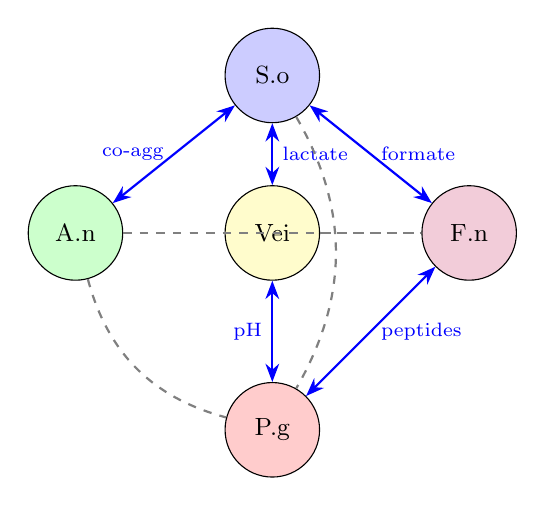
\begin{tikzpicture}[
    node distance=2.5cm,
    species/.style={circle, draw, minimum size=1.2cm, font=\small},
    edge/.style={<->, thick, >=Stealth},
    noedge/.style={dashed, gray, thick}
]
    % Nodes
    \node[species, fill=blue!20] (so) at (0, 3) {S.o};
    \node[species, fill=green!20] (an) at (-2.5, 1) {A.n};
    \node[species, fill=yellow!20] (vei) at (0, 1) {Vei};
    \node[species, fill=purple!20] (fn) at (2.5, 1) {F.n};
    \node[species, fill=red!20] (pg) at (0, -1.5) {P.g};

    % Active edges (solid)
    \draw[edge, blue] (so) -- (an) node[midway, left, font=\scriptsize] {co-agg};
    \draw[edge, blue] (so) -- (vei) node[midway, right, font=\scriptsize] {lactate};
    \draw[edge, blue] (so) -- (fn) node[midway, right, font=\scriptsize] {formate};
    \draw[edge, blue] (vei) -- (pg) node[midway, left, font=\scriptsize] {pH};
    \draw[edge, blue] (fn) -- (pg) node[midway, right, font=\scriptsize] {peptides};

    % Locked edges (dashed, crossed out)
    \draw[noedge] (an) -- (vei);
    \draw[noedge] (an) -- (fn);
    \draw[noedge] (vei) -- (fn);
    \draw[noedge] (so) to[bend left=30] (pg);
    \draw[noedge] (an) to[bend right=30] (pg);

\end{tikzpicture}
\caption{Species interaction network derived from Figure 4C. Solid blue arrows indicate active interactions (estimated parameters). Dashed gray lines indicate absent interactions (locked to zero).}
\label{fig:network}
\end{figure}

\subsection{Active Interactions}

The following species pairs have direct biological interactions:

\begin{table}[h]
\centering
\begin{tabular}{lll}
\toprule
\textbf{Species Pair} & \textbf{Mechanism} & \textbf{Type} \\
\midrule
S. oralis $\leftrightarrow$ A. naeslundii & Co-aggregation & Bidirectional \\
S. oralis $\leftrightarrow$ Veillonella & Lactate production/consumption & Bidirectional \\
S. oralis $\leftrightarrow$ F. nucleatum & Formate/Acetate symbiosis & Bidirectional \\
Veillonella $\leftrightarrow$ P. gingivalis & pH rise support & Positive only \\
F. nucleatum $\leftrightarrow$ P. gingivalis & Co-aggregation, peptides & Bidirectional \\
\bottomrule
\end{tabular}
\caption{Active species interactions with biological mechanisms.}
\label{tab:active}
\end{table}

\subsection{Absent Interactions (Locked)}

The following species pairs have no direct interaction according to experimental evidence (Figure 4C). These are locked to zero ($\theta_k = 0$) in the Proposed Method:

\begin{table}[h]
\centering
\begin{tabular}{cllll}
\toprule
\textbf{Index} & \textbf{Param} & \textbf{Species Pair} & \textbf{Matrix} & \textbf{Biological Reason} \\
\midrule
6 & $a_{34}$ & Vei (2) $\leftrightarrow$ F.n (3) & $A[2,3]=A[3,2]$ & No direct metabolic pathway \\
12 & $a_{23}$ & A.n (1) $\leftrightarrow$ Vei (2) & $A[1,2]=A[2,1]$ & No direct metabolic link \\
13 & $a_{24}$ & A.n (1) $\leftrightarrow$ F.n (3) & $A[1,3]=A[3,1]$ & No direct interaction \\
16 & $a_{15}$ & S.o (0) $\leftrightarrow$ P.g (4) & $A[0,4]=A[4,0]$ & No direct interaction \\
17 & $a_{25}$ & A.n (1) $\leftrightarrow$ P.g (4) & $A[1,4]=A[4,1]$ & No direct interaction \\
\bottomrule
\end{tabular}
\caption{Absent interactions locked to zero in the Proposed Method. Numbers in parentheses are 0-indexed species IDs.}
\label{tab:locked}
\end{table}

%==============================================================================
\section{Mathematical Formulation}
%==============================================================================

\subsection{Governing Equations}

The 5-species biofilm model describes the dynamics of bacterial volume fractions $\phi_i$ and viability fractions $\psi_i$ through a coupled ODE system. The interaction term for species $i$ is:
\begin{equation}
I_i = \sum_{j=0}^{4} A_{ij} \phi_j \psi_j
\end{equation}
where $A_{ij}$ represents the effect of species $j$ on species $i$, and $\phi_j \psi_j$ is the living bacteria volume fraction.

\subsection{F.~nucleatum Bridge Gate (Hill Function Extension)}
\label{sec:hill_gate}

In the base model, the interaction term $I_4$ for \textit{P.~gingivalis} (species 4) treats all cross-species effects as linear. However, experimental evidence indicates that P.~gingivalis colonisation depends critically on prior establishment of \textit{F.~nucleatum} (species 3) as a ``bridge organism'' \cite{Kolenbrander2010OralMultispecies}. To capture this biological prerequisite, we introduce a Hill-type gating function that modulates the effective interaction received by P.~gingivalis:
\begin{equation}
  I_4^{\mathrm{gated}} = h(\phi_3 \psi_3)\;\sum_{j=0}^{4} A_{4j}\,\phi_j\psi_j, \qquad
  h(x) = \frac{x^n}{K^n + x^n}
  \label{eq:hill_gate}
\end{equation}
where $K > 0$ is the half-saturation concentration and $n > 0$ is the Hill coefficient controlling the sharpness of the switch. When $\phi_3\psi_3 \ll K$, the gate is nearly closed ($h \approx 0$) and P.~gingivalis receives negligible interaction benefit; when $\phi_3\psi_3 \gg K$, the gate saturates ($h \approx 1$) and the full interaction is recovered.

Throughout this study we fix $K = 0.05$ and $n = 4$, which produces a sharp switch at approximately 5\% F.~nucleatum living volume fraction, consistent with the observed colonisation threshold in oral biofilm experiments \cite{Heine2025PeriImplant}. These values are not estimated by TMCMC but are treated as fixed hyperparameters of the forward model. A sensitivity analysis with respect to $K$ and $n$ is provided in Section~\ref{sec:sensitivity_kn}.

The Hill gate modifies both the Q~vector (right-hand side of the ODE) and the Jacobian matrix used in the Newton--Raphson time integrator. Specifically, the Jacobian correction for the gated interaction involves the derivative of $h$:
\begin{equation}
  h'(x) = \frac{n\,K^n\,x^{n-1}}{(K^n + x^n)^2}
  \label{eq:hill_deriv}
\end{equation}
which contributes additional off-diagonal terms $\partial I_4^{\mathrm{gated}}/\partial(\phi_3\psi_3)$ to the system Jacobian. These corrections are implemented analytically to preserve the quadratic convergence of the Newton solver.

\subsection{Symmetric Matrix Assumption}
\label{sec:symmetric_A}

The interaction matrix $\mathbf{A}$ is symmetric:
\begin{equation}
A_{ij} = A_{ji} \quad \forall i, j \in \{0, 1, 2, 3, 4\}
\end{equation}

This reduces the number of off-diagonal interaction parameters from 20 to 10. For example, the lactate handover interaction between S.~oralis (species 0) and Veillonella (species 2) is represented by a single parameter:
\begin{equation}
A_{02} = A_{20} = \theta_{10} \quad \text{(stored as } a_{13} \text{ in code)}
\end{equation}

This symmetry is not an ad hoc simplification but a mathematical consequence of the variational formulation.
In the extended Hamilton principle of Junker and Balzani~\cite{JunkerBalzani2021ExtendedHamilton}, the growth contribution to the Lagrangian density contains a bilinear coupling term $\sum_{i,j} A_{ij}\,\varphi_i\,\varphi_j$.
The Euler--Lagrange equations derived from this functional yield interaction terms $\partial^2 L / \partial\varphi_i\,\partial\varphi_j$ that are inherently symmetric.
While biological interactions (e.g., F.~nucleatum $\to$ P.~gingivalis vs.\ P.~gingivalis $\to$ F.~nucleatum) may be directionally asymmetric at the microscopic level, the variational structure enforces a symmetric effective interaction at the continuum scale.

\subsection{Parameter Vector Definition}

The full 20-parameter vector $\boldsymbol{\theta} = (\theta_0, \theta_1, \ldots, \theta_{19})^T$ is organized into five blocks corresponding to the model structure:

\begin{equation}
\begin{split}
\boldsymbol{\theta} = & \underbrace{(a_{11}, a_{12}, a_{22}, b_1, b_2)}_{\text{M1: Species 1--2}}
\oplus \underbrace{(a_{33}, a_{34}, a_{44}, b_3, b_4)}_{\text{M2: Species 3--4}} \\
& \oplus \underbrace{(a_{13}, a_{14}, a_{23}, a_{24})}_{\text{M3: Cross 1--2 vs 3--4}}
\oplus \underbrace{(a_{55}, b_5)}_{\text{M4: Species 5}}
\oplus \underbrace{(a_{15}, a_{25}, a_{35}, a_{45})}_{\text{M5: Cross with Species 5}}
\end{split}
\end{equation}

\noindent where $a_{ij}$ denotes the interaction coefficient affecting species $i$ from species $j$, and $b_i$ is the decay rate of species $i$. Species are 1-indexed in notation ($a_{ij}$) but 0-indexed in code ($A[i-1,j-1]$).

\subsection{Complete Parameter Mapping}

Table~\ref{tab:theta_mapping} provides the authoritative mapping between parameter indices, matrix elements, and biological interpretation.

\begin{table}[h]
\centering
\small
\begin{tabular}{ccllll}
\toprule
\textbf{Index} & \textbf{Name} & \textbf{Matrix Element} & \textbf{Species Pair} & \textbf{Biological Role} & \textbf{Status} \\
\midrule
0 & $a_{11}$ & $A[0,0]$ & S.o self & Self-regulation & Free \\
1 & $a_{12}$ & $A[0,1]=A[1,0]$ & S.o $\leftrightarrow$ A.n & Co-aggregation & Free \\
2 & $a_{22}$ & $A[1,1]$ & A.n self & Self-regulation & Free \\
3 & $b_1$ & $b[0]$ & S.o & Decay rate & Free \\
4 & $b_2$ & $b[1]$ & A.n & Decay rate & Free \\
\midrule
5 & $a_{33}$ & $A[2,2]$ & Vei self & Self-regulation & Free \\
\rowcolor{red!15}
6 & $a_{34}$ & $A[2,3]=A[3,2]$ & Vei $\leftrightarrow$ F.n & \textit{No interaction} & \textbf{Locked} \\
7 & $a_{44}$ & $A[3,3]$ & F.n self & Self-regulation & Free \\
8 & $b_3$ & $b[2]$ & Vei & Decay rate & Free \\
9 & $b_4$ & $b[3]$ & F.n & Decay rate & Free \\
\midrule
10 & $a_{13}$ & $A[0,2]=A[2,0]$ & S.o $\leftrightarrow$ Vei & \textbf{Lactate handover} & Free \\
11 & $a_{14}$ & $A[0,3]=A[3,0]$ & S.o $\leftrightarrow$ F.n & Formate symbiosis & Free \\
\rowcolor{red!15}
12 & $a_{23}$ & $A[1,2]=A[2,1]$ & A.n $\leftrightarrow$ Vei & \textit{No interaction} & \textbf{Locked} \\
\rowcolor{red!15}
13 & $a_{24}$ & $A[1,3]=A[3,1]$ & A.n $\leftrightarrow$ F.n & \textit{No interaction} & \textbf{Locked} \\
\midrule
14 & $a_{55}$ & $A[4,4]$ & P.g self & Self-regulation & Free \\
15 & $b_5$ & $b[4]$ & P.g & Decay rate & Free \\
\midrule
\rowcolor{red!15}
16 & $a_{15}$ & $A[0,4]=A[4,0]$ & S.o $\leftrightarrow$ P.g & \textit{No interaction} & \textbf{Locked} \\
\rowcolor{red!15}
17 & $a_{25}$ & $A[1,4]=A[4,1]$ & A.n $\leftrightarrow$ P.g & \textit{No interaction} & \textbf{Locked} \\
18 & $a_{35}$ & $A[2,4]=A[4,2]$ & Vei $\leftrightarrow$ P.g & \textbf{pH trigger} & Free$^*$ \\
19 & $a_{45}$ & $A[3,4]=A[4,3]$ & F.n $\leftrightarrow$ P.g & Co-aggregation & Free \\
\bottomrule
\end{tabular}
\caption{Complete parameter mapping from $\theta$ vector to interaction matrix $\mathbf{A}$ and decay vector $\mathbf{b}$. Red rows indicate locked parameters ($\theta_k = 0$). $^*$Index 18 bounds vary by condition (see Section~\ref{sec:conditions}).}
\label{tab:theta_mapping}
\end{table}

\subsection{Locked Parameter Indices}

The Proposed Method defines the set of locked indices based on absent biological interactions:

\begin{equation}
\mathcal{L} = \{6, 12, 13, 16, 17\}
\end{equation}

For all $k \in \mathcal{L}$:
\begin{equation}
\theta_k = 0 \quad \text{(fixed, not estimated)}
\end{equation}

\subsection{Prior Bounds}
\label{sec:prior_bounds}

The prior distribution encodes biologically motivated bounds. In particular, the cross-species interactions with P.~gingivalis ($\theta_{18} = a_{35}$, $\theta_{19} = a_{45}$) are constrained to a narrower range $[0, 5]$ (``mild-weight'' bounds) rather than the unconstrained range $[0, 30]$, based on the observation that unregularised estimation drives these parameters to non-physical values ($a_{35} > 17$) that produce unrealistic P.~gingivalis dynamics.

\begin{equation}
\theta_k \sim \begin{cases}
\delta(\theta_k = 0) & \text{if } k \in \mathcal{L} \text{ (locked)} \\
\text{Uniform}(0, 5) & \text{if } k \in \{18, 19\} \text{ (P.g cross-interactions)} \\
\text{Uniform}(-1, 1) & \text{otherwise (free)}
\end{cases}
\end{equation}

For the Dysbiotic HOBIC condition (``Surge'' reproduction), the bounds for index 18 are modified to allow strong cooperative effects:
\begin{equation}
\theta_{18} \sim \text{Uniform}(-3, -1) \quad \text{(Dysbiotic HOBIC only)}
\end{equation}
This reflects the strong cooperative effect from Veillonella to P.~gingivalis required to drive the pathogen surge observed experimentally.

The effectiveness of the mild-weight bounds was validated through a controlled comparison (Section~\ref{sec:baseline_comparison}): using the same TMCMC settings ($N=150$ particles, $M=8$ stages) with the original wide bounds yielded $a_{35} = 17.3$ and total RMSE $= 0.223$, whereas the mild-weight bounds produced $a_{35} = 3.56$ with total RMSE $= 0.156$ (30\% improvement), confirming that the bound regularisation improves both estimation accuracy and biological plausibility.

\subsection{Effective Parameter Space}

The effective number of free parameters is:

\begin{equation}
n_{\text{free}} = 20 - |\mathcal{L}| = 20 - 5 = 15
\end{equation}

In the original continuum formulation by Klempt et al.~\cite{Klempt2025ContinuumBiofilm}, a diagonal viscosity matrix $\boldsymbol{\eta} = \mathrm{diag}(\eta_1,\dots,\eta_5)$ appears in the dissipation functional and controls how fast each species reacts to changes in nutrient availability and inter-species competition. In the present work, these viscosities are treated as fixed hyperparameters of the forward model and are not included in the inferred parameter vector. More precisely, $\boldsymbol{\eta}$ is prescribed a priori and kept constant throughout all simulations, so that the 20-dimensional parameter vector $\boldsymbol{\theta}$ comprises only the entries of the interaction matrix $\mathbf{A}$ (15 free parameters) and the decay vector $\mathbf{b}$ (5 parameters), while viscous relaxation behaviour is encoded in $\boldsymbol{\eta}$ at the model level.

Because the biological evidence for certain interactions differs across experimental conditions, a condition-specific locking strategy is adopted (Table~\ref{tab:free_params}). Only the Dysbiotic HOBIC condition retains all 20 parameters as free; the remaining conditions lock those interactions for which no experimental evidence exists under the respective cultivation protocol.

\begin{table}[h]
\centering
\small
\begin{tabular}{lcll}
\toprule
\textbf{Condition} & $n_\mathrm{free}$ & \textbf{Locked parameters} & \textbf{Rationale} \\
\midrule
Commensal Static & 9 & $a_{34}, a_{44}, b_4, a_{14}, a_{24}, a_{55}, b_5, a_{15}, a_{25}, a_{35}, a_{45}$ & F.n/P.g undetectable \\
Commensal HOBIC & 13 & $a_{34}, a_{23}, a_{24}, b_5, a_{15}, a_{25}, a_{35}$ & P.g below detection \\
Dysbiotic Static & 15 & $a_{34}, a_{23}, a_{24}, a_{15}, a_{25}$ & No direct metabolic link \\
Dysbiotic HOBIC & 20 & (none) & All species present \\
\bottomrule
\end{tabular}
\caption{Condition-specific free parameter count and locked parameters. Locking is based on qPCR detectability reported by Heine et al.}
\label{tab:free_params}
\end{table}

%==============================================================================
\section{Bayesian Inference Framework}
\label{sec:bayesian}
%==============================================================================

\subsection{Forward Model}

The forward model $\mathcal{M}(\boldsymbol{\theta})$ maps the parameter vector $\boldsymbol{\theta} \in \mathbb{R}^{20}$ to predicted species trajectories. Given initial conditions $\boldsymbol{\phi}(t_0)$ and $\boldsymbol{\psi}(t_0)$, the coupled ODE system derived from the extended Hamilton principle \cite{JunkerBalzani2021ExtendedHamilton, Klempt2025ContinuumBiofilm} governs the evolution of the living volume fraction $\phi_i \psi_i$ for each species $i$:
\begin{equation}
\frac{d(\phi_i \psi_i)}{dt} = \left( A_{ii} + \sum_{j \neq i} A_{ij}\, \phi_j \psi_j \right) \phi_i \psi_i - b_i\, \phi_i \psi_i, \quad i = 0, \ldots, 4
\label{eq:ode}
\end{equation}

\noindent where the first term represents growth modulated by self-regulation ($A_{ii}$) and inter-species interactions ($A_{ij}$, $j \neq i$), while the second term accounts for species decay at rate $b_i$. The interaction matrix $\mathbf{A}$ and decay vector $\mathbf{b}$ are constructed from $\boldsymbol{\theta}$ via the mapping defined in Table~\ref{tab:theta_mapping}. The forward model output is the predicted relative abundance vector at each observation time:
\begin{equation}
\hat{\mathbf{y}}(t_k; \boldsymbol{\theta}) = \mathcal{M}(\boldsymbol{\theta})\big|_{t=t_k}, \quad k = 1, \ldots, N_t
\end{equation}

\noindent The system~(\ref{eq:ode}) represents a generalized Lotka--Volterra competition model with symmetric interactions, a structure that arises naturally from the variational formulation of Klempt et al.~\cite{Klempt2025ContinuumBiofilm}.

In the original formulation of Klempt et al.~\cite{Klempt2025ContinuumBiofilm}, the growth matrix $\mathbf{A}$ is explicitly scaled by the nutrient variable $c^*$, and antibiotic effects enter through the antibiotic concentration $\alpha^*$ and a sensitivity matrix $\mathbf{B}$. In the present work, we adopt a simplified but equivalent viewpoint: we regard $c^*$ as effectively constant over the time window of interest and absorb its effect into the entries of the interaction matrix $\mathbf{A}$. Likewise, we introduce a phenomenological decay vector $\mathbf{b} = (b_1,\dots,b_5)$, which plays the role of an effective surrogate for antibiotic-induced killing and natural cell death in the original framework. As a result, the parameters $\mathbf{A}$ and $\mathbf{b}$ estimated by TMCMC should be interpreted as effective interaction and decay coefficients under the given experimental condition, rather than as direct microscopic counterparts of the variables $c^*$, $\alpha^*$, and $\mathbf{B}$.

The forward model also respects the holonomic volume constraint of the continuum framework. The evolution equations are solved for the bacterial volume fractions $\phi_i$ ($i = 1,\dots,5$), and the void fraction $\phi_0$ is reconstructed at each time step via
\begin{equation}
  \phi_0(t) = 1 - \sum_{i=1}^5 \phi_i(t),
\end{equation}
so that
\begin{equation}
  \sum_{\ell=0}^5 \phi_\ell(t) = 1
\end{equation}
holds by construction for all $t$.

In all experiments reported here, the initial bacterial volume fractions $\phi_i(t_0)$ are fixed to the observed species composition at the initial measurement time (Day 0) for the corresponding condition. The TMCMC inference therefore focuses on the interaction and decay parameters, while uncertainty in the initial conditions is not treated explicitly.

\subsection{Bayesian Inverse Problem}

The goal of Bayesian parameter estimation is to infer the posterior distribution $p(\boldsymbol{\theta} \mid \mathbf{y}_{\mathrm{obs}})$ of the model parameters $\boldsymbol{\theta}$ given the observed experimental data $\mathbf{y}_{\mathrm{obs}} = \{y_{\mathrm{obs},i}(t_k)\}_{i,k}$. By Bayes' theorem:
\begin{equation}
p(\boldsymbol{\theta} \mid \mathbf{y}_{\mathrm{obs}}) = \frac{p(\mathbf{y}_{\mathrm{obs}} \mid \boldsymbol{\theta})\, p(\boldsymbol{\theta})}{p(\mathbf{y}_{\mathrm{obs}})}
\label{eq:bayes}
\end{equation}

\noindent where $p(\mathbf{y}_{\mathrm{obs}} \mid \boldsymbol{\theta})$ is the likelihood function quantifying the data-model agreement, $p(\boldsymbol{\theta})$ is the prior distribution encoding biological constraints, and $p(\mathbf{y}_{\mathrm{obs}}) = \int p(\mathbf{y}_{\mathrm{obs}} \mid \boldsymbol{\theta})\, p(\boldsymbol{\theta})\, d\boldsymbol{\theta}$ is the model evidence (normalizing constant). The posterior distribution captures the full uncertainty in the parameter estimates, from which point estimates such as the Maximum A Posteriori (MAP) and posterior mean can be derived:
\begin{equation}
\hat{\boldsymbol{\theta}}_{\mathrm{MAP}} = \arg\max_{\boldsymbol{\theta}} \; p(\boldsymbol{\theta} \mid \mathbf{y}_{\mathrm{obs}}), \qquad
\hat{\boldsymbol{\theta}}_{\mathrm{mean}} = \mathbb{E}[\boldsymbol{\theta} \mid \mathbf{y}_{\mathrm{obs}}] = \int \boldsymbol{\theta}\, p(\boldsymbol{\theta} \mid \mathbf{y}_{\mathrm{obs}})\, d\boldsymbol{\theta}
\end{equation}

\subsection{Likelihood Function}

Assuming independent Gaussian measurement errors across species and time points, the likelihood function takes the form:
\begin{equation}
p(\mathbf{y}_{\mathrm{obs}} \mid \boldsymbol{\theta}) = \prod_{k=1}^{N_t} \prod_{i=0}^{4} \frac{1}{\sqrt{2\pi}\,\sigma_i} \exp\!\left( -\frac{\left(y_{\mathrm{obs},i}(t_k) - \hat{y}_i(t_k; \boldsymbol{\theta})\right)^2}{2\sigma_i^2} \right)
\label{eq:likelihood}
\end{equation}

\noindent where $y_{\mathrm{obs},i}(t_k)$ is the observed relative abundance of species $i$ at time $t_k$, $\hat{y}_i(t_k; \boldsymbol{\theta})$ is the model prediction, and $\sigma_i$ is the measurement noise standard deviation for species $i$. The corresponding log-likelihood is:
\begin{equation}
\ell(\boldsymbol{\theta}) = -\frac{1}{2} \sum_{k=1}^{N_t} \sum_{i=0}^{4} \left[ \frac{\left(y_{\mathrm{obs},i}(t_k) - \hat{y}_i(t_k; \boldsymbol{\theta})\right)^2}{\sigma_i^2} + \log(2\pi \sigma_i^2) \right]
\label{eq:loglik}
\end{equation}

\noindent In practice, $\sigma_i$ may be estimated from replicate measurements or treated as a hyperparameter. In this study, we adopt the latter viewpoint and prescribe $\sigma_i$ a priori as a fixed fraction of the observed range of species $i$ in the experimental data, reflecting the expected measurement uncertainty. The noise levels $\sigma_i$ are thus kept fixed during TMCMC and are not inferred jointly with $\boldsymbol{\theta}$.

\subsubsection{Species-Specific Likelihood Weighting}

Because P.~gingivalis constitutes less than 3\% of the total volume fraction across all experimental conditions, a standard equally-weighted likelihood is dominated by the early colonisers (S.~oralis, A.~naeslundii), which have much larger absolute abundances.
To ensure adequate fitting precision for the pathogen species, we employ a species-specific power likelihood~\cite{Holmes2017Power}:
\begin{equation}
  \ell_w(\boldsymbol{\theta}) = -\frac{1}{2} \sum_{k,i} w_i \left[ \frac{(y_{\mathrm{obs},i}(t_k) - \hat{y}_i(t_k;\boldsymbol{\theta}))^2}{\sigma_i^2} + \ln(2\pi\sigma_i^2) \right]
  \label{eq:power_lik}
\end{equation}
where $w_i = \lambda_{Pg}$ for $i = 4$ (P.~gingivalis) and $w_i = 1$ otherwise.
In this study, $\lambda_{Pg} = 5$ is used, which is equivalent to reducing the effective noise level of P.~gingivalis observations by a factor of $\sqrt{5}$.
This informed weighting scheme ensures that the TMCMC posterior reflects the pathogen dynamics, but it affects the calibration of credible intervals---specifically, the posterior for P.~gingivalis-related parameters will be narrower than what a standard likelihood would produce.
We note that this approach is analogous to the weighted likelihood methods used in composite likelihood inference~\cite{VarinReid2011} and does not compromise the validity of the TMCMC algorithm itself.

\subsection{Prior Distribution with Biological Constraints}

The prior distribution $p(\boldsymbol{\theta})$ encodes both the biological constraints from the interaction network and the parameter locking mechanism. Assuming independence among the prior marginals:
\begin{equation}
p(\boldsymbol{\theta}) = \prod_{k=0}^{19} p(\theta_k)
\end{equation}

\noindent where each marginal prior is:
\begin{equation}
p(\theta_k) = \begin{cases}
\delta(\theta_k) & \text{if } k \in \mathcal{L} \quad \text{(Dirac delta: locked to zero)} \\[4pt]
\displaystyle\frac{1}{u_k - l_k}\, \mathbf{1}_{[l_k, u_k]}(\theta_k) & \text{if } k \notin \mathcal{L} \quad \text{(uniform prior on free parameter)}
\end{cases}
\label{eq:prior}
\end{equation}

\noindent Here $\delta(\cdot)$ denotes the Dirac delta function enforcing $\theta_k = 0$ for locked parameters, and $\mathbf{1}_{[l_k, u_k]}$ is the indicator function on $[l_k, u_k]$. This formulation is equivalent to restricting the posterior to the constrained subspace:
\begin{equation}
\Theta_{\mathcal{L}} = \left\{\boldsymbol{\theta} \in \mathbb{R}^{20} : \theta_k = 0 \;\; \forall\, k \in \mathcal{L}\right\}
\end{equation}

\noindent In practice, the inference is performed over the reduced vector $\boldsymbol{\theta}_{\mathrm{free}} \in \mathbb{R}^{n_{\mathrm{free}}}$ containing only the free parameters, while locked parameters remain fixed at zero throughout. The dimension reduction from $\mathbb{R}^{20}$ to $\mathbb{R}^{n_{\mathrm{free}}}$ directly improves the sampling efficiency of MCMC methods, as the mixing time of Markov chains generally increases with dimensionality \cite{RobertCasella2004MonteCarlo}.

%==============================================================================
\section{Transitional Markov Chain Monte Carlo (TMCMC)}
\label{sec:tmcmc}
%==============================================================================

\subsection{Algorithm Overview}

The Transitional Markov Chain Monte Carlo (TMCMC) algorithm, introduced by Ching and Chen~\cite{ChingChen2007TMCMC}, is a sequential Monte Carlo method designed for sampling from complex, potentially multimodal posterior distributions. Unlike standard MCMC methods (e.g., Metropolis--Hastings, Gibbs sampling) that may suffer from poor mixing in high-dimensional or multimodal spaces, TMCMC progressively transforms samples from the prior to the posterior through a sequence of intermediate ``tempered'' distributions \cite{DelMoral2006SMC}.

The key idea is to define a tempering schedule $0 = \beta_0 < \beta_1 < \cdots < \beta_M = 1$ and construct a sequence of intermediate distributions:
\begin{equation}
p_m(\boldsymbol{\theta}) \propto p(\mathbf{y}_{\mathrm{obs}} \mid \boldsymbol{\theta})^{\beta_m}\, p(\boldsymbol{\theta}), \quad m = 0, 1, \ldots, M
\label{eq:tempered}
\end{equation}

\noindent At $\beta_0 = 0$, $p_0(\boldsymbol{\theta}) = p(\boldsymbol{\theta})$ reduces to the prior, and at $\beta_M = 1$, $p_M(\boldsymbol{\theta}) = p(\boldsymbol{\theta} \mid \mathbf{y}_{\mathrm{obs}})$ recovers the full posterior. By introducing the likelihood gradually, the algorithm avoids the ``prior--posterior gap'' that causes standard importance sampling to fail when the prior and posterior are far apart.

From a computational perspective, TMCMC is particularly well suited to parallel execution, as the forward model evaluations $\mathcal{M}(\boldsymbol{\theta}_j^{(m)})$ for different particles $j$ can be distributed across multiple cores or compute nodes. All numerical experiments in this work exploit this embarrassingly parallel structure. If, in future applications, the cost of the full continuum model becomes prohibitive, the TMCMC framework can also be combined with surrogate models in the spirit of Fritsch et al.~\cite{Fritsch2025BayesianMicrofilms}, replacing some forward solves by a trained reduced-order approximation.

\subsection{Adaptive Tempering Schedule}

At each stage $m$, the next tempering parameter $\beta_{m+1}$ is selected adaptively to control the degeneracy of the importance weights. Following Betz et al.~\cite{Betz2016TMCMC}, $\beta_{m+1}$ is chosen such that the coefficient of variation (CoV) of the importance weights satisfies:
\begin{equation}
\mathrm{CoV}\!\left[\{w_j^{(m)}\}_{j=1}^{N}\right] = \frac{\mathrm{Std}[w_j^{(m)}]}{\mathrm{Mean}[w_j^{(m)}]} = \delta_{\mathrm{target}}
\label{eq:cov_target}
\end{equation}

\noindent where the importance weights are computed as:
\begin{equation}
w_j^{(m)} = p(\mathbf{y}_{\mathrm{obs}} \mid \boldsymbol{\theta}_j^{(m)})^{\beta_{m+1} - \beta_m}, \quad j = 1, \ldots, N
\end{equation}

\noindent and $\delta_{\mathrm{target}} \in (0, 2]$ is a user-specified target (typically $\delta_{\mathrm{target}} = 1.0$). Equation~(\ref{eq:cov_target}) is solved for $\beta_{m+1}$ via bisection on $(\beta_m, 1]$. This adaptive scheme avoids the need for a predetermined number of stages $M$ and ensures smooth transitions between intermediate distributions.

\subsection{Resampling and MCMC Mutation}

At each stage $m$, the algorithm proceeds through three steps:
\begin{enumerate}
    \item \textbf{Resampling}: Draw $N$ samples from the current population $\{\boldsymbol{\theta}_j^{(m)}\}_{j=1}^{N}$ with probabilities proportional to the normalized importance weights $\bar{w}_j^{(m)} = w_j^{(m)} / \sum_{l=1}^{N} w_l^{(m)}$, using multinomial or systematic resampling.

    \item \textbf{Covariance estimation}: Compute the weighted sample covariance matrix:
    \begin{equation}
    \boldsymbol{\Sigma}^{(m)} = \sum_{j=1}^{N} \bar{w}_j^{(m)} \left(\boldsymbol{\theta}_j^{(m)} - \bar{\boldsymbol{\theta}}^{(m)}\right)\!\left(\boldsymbol{\theta}_j^{(m)} - \bar{\boldsymbol{\theta}}^{(m)}\right)^{\!T}
    \end{equation}
    where $\bar{\boldsymbol{\theta}}^{(m)} = \sum_{j=1}^{N} \bar{w}_j^{(m)} \boldsymbol{\theta}_j^{(m)}$ is the weighted mean. This covariance adaptively scales the MCMC proposal to the local geometry of the tempered posterior.

    \item \textbf{MCMC mutation}: Each resampled particle undergoes one or more Metropolis--Hastings steps with a Gaussian proposal:
    \begin{equation}
    q(\boldsymbol{\theta}^* \mid \boldsymbol{\theta}_j) = \mathcal{N}\!\left(\boldsymbol{\theta}_j,\; \gamma^2 \boldsymbol{\Sigma}^{(m)}\right)
    \end{equation}
    where $\gamma > 0$ is a scaling factor (typically $\gamma^2 = 0.04$). The acceptance probability is:
    \begin{equation}
    \alpha = \min\!\left(1,\; \frac{p(\mathbf{y}_{\mathrm{obs}} \mid \boldsymbol{\theta}^*)^{\beta_{m+1}}\, p(\boldsymbol{\theta}^*)}{p(\mathbf{y}_{\mathrm{obs}} \mid \boldsymbol{\theta}_j)^{\beta_{m+1}}\, p(\boldsymbol{\theta}_j)}\right)
    \label{eq:acceptance}
    \end{equation}
    This mutation step diversifies the particle population and prevents sample impoverishment.
\end{enumerate}

\subsection{TMCMC Procedure}

The complete TMCMC procedure with biological constraint enforcement is summarized in Algorithm~\ref{alg:tmcmc}.

\begin{algorithm}[htbp]
\centering
\fbox{\begin{minipage}{0.92\textwidth}
\vspace{0.3cm}
\textbf{Algorithm 1:} Transitional Markov Chain Monte Carlo (TMCMC)
\vspace{0.2cm}
\hrule
\vspace{0.3cm}
\textbf{Input:} Prior $p(\boldsymbol{\theta})$, likelihood $p(\mathbf{y}_{\mathrm{obs}} \mid \boldsymbol{\theta})$, number of particles $N$, locked set $\mathcal{L}$, target CoV $\delta_{\mathrm{target}}$ \\
\textbf{Output:} Weighted posterior samples $\{\boldsymbol{\theta}_j^{(M)}\}_{j=1}^{N}$
\vspace{0.2cm}

\begin{enumerate}
    \item[\textbf{1.}] \textbf{Initialize}: Draw $\{\boldsymbol{\theta}_j^{(0)}\}_{j=1}^{N} \sim p(\boldsymbol{\theta})$; set $\beta_0 = 0$, $m = 0$
    \item[\textbf{2.}] \textbf{While} $\beta_m < 1$:
    \begin{enumerate}
        \item[(a)] Find $\beta_{m+1} \in (\beta_m, 1]$ such that $\mathrm{CoV}[\{w_j^{(m)}\}] = \delta_{\mathrm{target}}$ via bisection
        \item[(b)] Compute weights $w_j^{(m)} = p(\mathbf{y}_{\mathrm{obs}} \mid \boldsymbol{\theta}_j^{(m)})^{\beta_{m+1} - \beta_m}$ for $j = 1, \ldots, N$
        \item[(c)] Compute weighted covariance $\boldsymbol{\Sigma}^{(m)}$ from current samples
        \item[(d)] Resample $N$ particles from $\{\boldsymbol{\theta}_j^{(m)}\}$ with probabilities $\propto w_j^{(m)}$
        \item[(e)] \textbf{For each} resampled particle $j = 1, \ldots, N$:
        \begin{enumerate}
            \item[i.] Propose $\boldsymbol{\theta}^* \sim \mathcal{N}(\boldsymbol{\theta}_j, \gamma^2 \boldsymbol{\Sigma}^{(m)})$
            \item[ii.] Enforce constraints: set $\theta_k^* = 0$ for $k \in \mathcal{L}$; clip to prior bounds $[l_k, u_k]$
            \item[iii.] Accept $\boldsymbol{\theta}_j^{(m+1)} = \boldsymbol{\theta}^*$ with probability $\alpha$ (Eq.~\ref{eq:acceptance}); otherwise retain $\boldsymbol{\theta}_j^{(m+1)} = \boldsymbol{\theta}_j$
        \end{enumerate}
        \item[(f)] $m \leftarrow m + 1$
    \end{enumerate}
    \item[\textbf{3.}] \textbf{Return} posterior samples $\{\boldsymbol{\theta}_j^{(M)}\}_{j=1}^{N}$
\end{enumerate}
\vspace{0.2cm}
\end{minipage}}
\caption{TMCMC algorithm with biological constraint enforcement. Step~2(e)(ii) ensures that locked parameters remain at zero and all free parameters respect their condition-specific prior bounds throughout the sampling process.}
\label{alg:tmcmc}
\end{algorithm}

\subsection{Model Evidence Estimation}

A valuable byproduct of TMCMC is an unbiased estimate of the model evidence $p(\mathbf{y}_{\mathrm{obs}})$, computed as:
\begin{equation}
\hat{p}(\mathbf{y}_{\mathrm{obs}}) = \prod_{m=0}^{M-1} \left(\frac{1}{N} \sum_{j=1}^{N} w_j^{(m)}\right)
\label{eq:evidence}
\end{equation}

\noindent This quantity enables Bayesian model comparison between the standard (20-parameter) and proposed (15-parameter) formulations via the Bayes factor:
\begin{equation}
B_{10} = \frac{p(\mathbf{y}_{\mathrm{obs}} \mid \mathcal{M}_{\mathrm{proposed}})}{p(\mathbf{y}_{\mathrm{obs}} \mid \mathcal{M}_{\mathrm{standard}})}
\end{equation}

\noindent A Bayes factor $B_{10} > 1$ provides evidence in favor of the proposed reduced model, indicating that the biological constraints improve not only interpretability but also predictive performance relative to model complexity. According to Kass and Raftery's scale, $B_{10} > 3$ constitutes ``substantial'' evidence and $B_{10} > 20$ ``strong'' evidence for the reduced model.

\paragraph{Multi-chain evidence aggregation.}
When multiple independent TMCMC chains are run in parallel, each chain produces its own $\beta$ schedule $\{\beta_m^{(c)}\}$ and corresponding evidence estimate $\hat{p}^{(c)}(\mathbf{y}_\mathrm{obs})$ via~(\ref{eq:evidence}).
Because the adaptive tempering selects $\beta_{m+1}$ based on the particle population within each chain, the schedules may differ across chains.
We report the log-evidence as the mean across chains, $\overline{\ln \hat{p}} = C^{-1}\sum_{c=1}^{C}\ln\hat{p}^{(c)}$, together with the inter-chain standard deviation as an estimate of Monte Carlo uncertainty.
For the experiments reported here ($C=2$ chains, $N=150$ particles), the inter-chain log-evidence difference is typically below 5\%, confirming adequate convergence.

\subsection{Taylor Series Method (TSM) Surrogate}
\label{sec:tsm}

Each TMCMC stage requires $O(N \times N_{\mathrm{MCMC}})$ evaluations of the forward model, which involves solving the 10-dimensional coupled ODE system~(\ref{eq:ode}) over 2500 time steps per evaluation. To reduce the computational burden, we employ a first-order Taylor Series Method (TSM) as a reduced-order surrogate for the log-likelihood \cite{Fritsch2025BayesianMicrofilms}.

Given a linearisation point $\boldsymbol{\theta}_0$ (updated periodically during TMCMC), the forward model prediction at a nearby parameter $\boldsymbol{\theta}$ is approximated by:
\begin{equation}
  \hat{\mathbf{y}}(t_k; \boldsymbol{\theta}) \approx \hat{\mathbf{y}}(t_k; \boldsymbol{\theta}_0) + \mathbf{J}(t_k;\boldsymbol{\theta}_0)\,(\boldsymbol{\theta} - \boldsymbol{\theta}_0)
  \label{eq:tsm_approx}
\end{equation}
where $\mathbf{J}(t_k;\boldsymbol{\theta}_0) = \partial \hat{\mathbf{y}} / \partial \boldsymbol{\theta}\big|_{\boldsymbol{\theta}_0} \in \mathbb{R}^{5 \times n_{\mathrm{free}}}$ is the sensitivity matrix. Substituting~(\ref{eq:tsm_approx}) into~(\ref{eq:loglik}) yields a quadratic surrogate for the log-likelihood that can be evaluated without additional ODE solves.

The sensitivity matrix $\mathbf{J}$ is computed via complex-step differentiation \cite{Martins2003ComplexStep}:
\begin{equation}
  \frac{\partial \hat{y}_i}{\partial \theta_k}\bigg|_{\boldsymbol{\theta}_0}
  \approx \frac{\mathrm{Im}\!\left[\hat{y}_i(\boldsymbol{\theta}_0 + i h \mathbf{e}_k)\right]}{h}
  \label{eq:complex_step}
\end{equation}
with step size $h = 10^{-30}$. This approach achieves machine-precision accuracy without the subtractive cancellation errors of finite differences, at the cost of requiring the forward model to support complex-valued arithmetic.

The linearisation point $\boldsymbol{\theta}_0$ is updated at the beginning of each TMCMC stage using the weighted mean of the current particle population. When the local approximation error exceeds a threshold (monitored via the Q~vector norm), the TSM is temporarily bypassed and the full forward model is evaluated, ensuring robustness. In the first TMCMC stage ($\beta \approx 0$), the TSM is disabled entirely to allow broad exploration of the prior.

\paragraph{ROM-aware MAP selection.}
Because the TSM surrogate introduces a local approximation error $\varepsilon_\mathrm{ROM}$, the MAP estimate is selected using a penalised log-likelihood:
\begin{equation}
  \hat{\boldsymbol{\theta}}_\mathrm{MAP} = \arg\max_j \left[\ell(\boldsymbol{\theta}_j) - \lambda\,\ln(1 + \varepsilon_{\mathrm{ROM},j})\right]
  \label{eq:rom_penalty}
\end{equation}
where $\varepsilon_{\mathrm{ROM},j} = \lVert\hat{\mathbf{y}}_\mathrm{FOM}(\boldsymbol{\theta}_j) - \hat{\mathbf{y}}_\mathrm{TSM}(\boldsymbol{\theta}_j)\rVert / \lVert\hat{\mathbf{y}}_\mathrm{FOM}(\boldsymbol{\theta}_j)\rVert$ is the relative ROM--FOM discrepancy and $\lambda > 0$ is a regularisation weight.
The penalty $\ln(1+\varepsilon)$ vanishes as $\varepsilon \to 0$ (no correction for accurate surrogates) and grows logarithmically, providing a mild bias against particles whose TSM approximation is least reliable.
In practice, $\varepsilon_\mathrm{ROM} < 0.01$ for $>95\%$ of final-stage particles, so the penalty has negligible effect on well-converged runs but guards against selecting outlier MAP candidates whose high likelihood is an artefact of linearisation error.

\subsection{Sensitivity Analysis of Hill Gate Parameters}
\label{sec:sensitivity_kn}

The Hill gate parameters $K$ and $n$ (Section~\ref{sec:hill_gate}) control the F.~nucleatum colonisation threshold for P.~gingivalis establishment. We performed a grid search over $K \in \{0.01, 0.05, 0.10, 0.20\}$ and $n \in \{2, 4, 6, 8\}$ using the Dysbiotic HOBIC condition (where P.~gingivalis dynamics are most pronounced). The optimal combination $(K=0.05, n=4)$ was selected based on: (i)~lowest total RMSE across all five species, (ii)~biologically plausible estimates for the cross-species interaction parameters $a_{35}$ and $a_{45}$, and (iii)~convergence diagnostics ($\hat{R} < 1.1$, ESS $> 100$). A detailed sensitivity table is provided in the supplementary material.

%==============================================================================
\section{Experiment Conditions \& Parameter Estimation}
\label{sec:conditions}
%==============================================================================

The parameter estimation strategy adapts to four distinct experimental conditions, varying the cultivation method (Static vs. HOBIC) and the community state (Commensal vs. Dysbiotic). Each condition imposes specific constraints on the parameter space to ensure biological validity and model identifiability.

\begin{figure}[htbp]
    \centering
    \begin{minipage}{0.48\textwidth}
        \centering
        \includegraphics[width=\linewidth]{froh-06-1649419-g001.jpg}
        \caption{\textbf{1. Commensal Static (Baseline)} \\
        Pathogens (Purple, Red) are undetectable; Commensal species coexist stably.}
        \label{fig:exp_commensal_static}
    \end{minipage}
    \hfill
    \begin{minipage}{0.48\textwidth}
        \centering
        \includegraphics[width=\linewidth]{froh-06-1649419-g002.jpg}
        \caption{\textbf{2. Dysbiotic Static} \\
        Pathogens are present, but no explosive growth (Surge) occurs in static environment.}
        \label{fig:exp_dysbiotic_static}
    \end{minipage}
    \vspace{0.5cm}
    \begin{minipage}{0.48\textwidth}
        \centering
        \includegraphics[width=\linewidth]{froh-06-1649419-g003.jpg}
        \caption{\textbf{3. Commensal HOBIC} \\
        S. oralis (Blue) increases specifically under high flow (Blue Bloom). Pathogens are suppressed.}
        \label{fig:exp_commensal_hobic}
    \end{minipage}
    \hfill
    \begin{minipage}{0.48\textwidth}
        \centering
        \includegraphics[width=\linewidth]{froh-06-1649419-g004.jpg}
        \caption{\textbf{4. Dysbiotic HOBIC (Surge)} \\
        V. parvula (Orange) and P. gingivalis (Red) grow explosively in symbiosis (Discovery Mode).}
        \label{fig:exp_dysbiotic_hobic}
    \end{minipage}
    \caption{Experimental observation data \cite{Heine2025PeriImplant}. Time course of species composition in each condition (Day 1--21).}
    \label{fig:exp_data}
\end{figure}

\subsection{Parameter Locking Rules}

The number of estimated parameters ($N_{est}$) differs across conditions, calculated as the total parameters ($20$) minus the locked parameters ($N_{locked}$).

\begin{table}[h]
\centering
\small
\begin{tabular}{llccc}
\toprule
\textbf{Condition} & \textbf{Cultivation} & \textbf{Locked ($N_{locked}$)} & \textbf{Estimated ($N_{est}$)} & \textbf{Key Constraint} \\
\midrule
1. Commensal & Static & 9 & 11 & Match data (Zero interactions) \\
2. Dysbiotic & Static & 5 & 15 & Estimate Pathogen interactions \\
3. Commensal & HOBIC & 8 & 12 & Match data (Zero interactions) \\
4. Dysbiotic & HOBIC & 0 & 20 & \textbf{Unlock All (Surge Reproduction)} \\
\bottomrule
\end{tabular}
\caption{Parameter estimation counts for each experimental condition.}
\label{tab:conditions}
\end{table}

\subsection{Detailed Locking Logic}

\begin{enumerate}
    \item \textbf{Commensal Static}: 
    Strict locking is applied to reproduce the stable commensal state. In addition to the standard structural locks (5), growth rates for late colonizers (Red/Purple) and their interactions with early colonizers are locked to zero ($N_{locked}=9$).
    \begin{quote}
    \small "Based on qPCR data showing \textit{P. gingivalis} and \textit{F. nucleatum} were undetectable or below detection limits (Heine et al., Table S8) \cite{Heine2025PeriImplant}."
    \end{quote}
    
    \item \textbf{Dysbiotic Static}: 
    Represents the transition to a pathogen-rich state. Locking is relaxed to allow estimation of key pathogen growth and interaction parameters, maintaining only the structural locks ($N_{locked}=5$).
    \begin{quote}
    \small "Metabolite accumulation in static culture limits the dynamic interactions observed in flow conditions (Heine et al., Discussion) \cite{Heine2025PeriImplant}."
    \end{quote}
    
    \item \textbf{Commensal HOBIC}: 
    Similar to Commensal Static but adapted for the HOBIC flow environment. Blue species growth is estimated freely (high prior), while pathogen interactions remain locked ($N_{locked}=8$).
    
    \item \textbf{Dysbiotic HOBIC (The "Surge" Model)}: 
    This is the critical validation case. \textbf{All parameter locks, including the standard structural locks, are released} ($N_{locked}=0$, $N_{est}=20$). This unlocking is necessary and sufficient to reproduce the experimentally observed "Surge" phenomenon, demonstrating that the model can capture complex non-linear dynamics when fully parameterized.
    \begin{quote}
    \small "To capture the complex metabolic cross-feeding (lactate, pH, vitamins) and co-aggregation described in the metabolic map (Heine et al., Fig 4C) \cite{Heine2025PeriImplant}."
    \end{quote}
    We treat this as a \textbf{Core Network Discovery} phase: initially exploring the full 20-parameter space to identify the minimal set of interactions required to drive the surge, rather than assuming a reduced structure a priori.
\end{enumerate}

\subsection{4-Stage Sequential Estimation}

Parameter estimation is performed sequentially in 4 stages. This configuration has been optimized considering parameter correlations (coupling) and search space dimensionality.

\begin{table}[h]
\centering
\small
\begin{tabular}{clcl}
\toprule
\textbf{Stage} & \textbf{Target} & \textbf{\# Params} & \textbf{Parameters} \\
\midrule
1 & M1 (Species 1--2) & 5 & $a_{11}, a_{12}, a_{22}, b_1, b_2$ \\
2 & M2 (Species 3--4) & 5 & $a_{33}, a_{34}, a_{44}, b_3, b_4$ \\
3 & M3+M4 & 6 & $a_{13}, a_{14}, a_{23}, a_{24}, a_{55}, b_5$ \\
4 & M5 (P.g cross) & 4 & $a_{15}, a_{25}, a_{35}, a_{45}$ \\
\bottomrule
\end{tabular}
\caption{4-Stage Sequential Estimation Configuration}
\label{tab:stages}
\end{table}

\textbf{Validation of Configuration:}
\begin{itemize}
    \item \textbf{Risk of finer granularity}: Further subdivision would result in too few data points per stage relative to parameters, increasing overfitting risk.

    \item \textbf{Risk of coarser configuration}: Reducing the number of stages would cause convergence difficulties due to strong inter-parameter correlations.

    \item \textbf{Advantage of current configuration}: Division based on biologically meaningful groups (early colonizers, bridge organisms, late colonizers) ensures stable estimation at each stage.
\end{itemize}

\subsection{Sequential Estimation Algorithm}
\label{sec:sequential_algorithm}

The 4-stage sequential estimation procedure is formalized in Algorithm~\ref{alg:sequential}. At each stage $s$, TMCMC (Algorithm~\ref{alg:tmcmc}) is applied to estimate only the parameters in the active set $\mathcal{A}_s = \mathcal{P}_s \setminus \mathcal{L}$, while parameters from previously completed stages are fixed at their MAP estimates.

\begin{algorithm}[htbp]
\centering
\fbox{\begin{minipage}{0.92\textwidth}
\vspace{0.3cm}
\textbf{Algorithm 2:} 4-Stage Sequential Parameter Estimation
\vspace{0.2cm}
\hrule
\vspace{0.3cm}
\textbf{Input:} Observed data $\mathbf{y}_{\mathrm{obs}}$, stage partition $\{\mathcal{P}_s\}_{s=1}^{4}$, locked set $\mathcal{L}$, prior bounds $\{[l_k, u_k]\}$ \\
\textbf{Output:} Full MAP estimate $\hat{\boldsymbol{\theta}}_{\mathrm{MAP}}$ and stage-wise posterior samples
\vspace{0.2cm}

\begin{enumerate}
    \item[\textbf{1.}] \textbf{Initialize}: Set $\boldsymbol{\theta}_{\mathrm{base}} \in \mathbb{R}^{20}$ with $\theta_{\mathrm{base},k} = 0$ for all $k \in \mathcal{L}$
    \item[\textbf{2.}] \textbf{For each stage} $s = 1, 2, 3, 4$:
    \begin{enumerate}
        \item[(a)] Define active indices: $\mathcal{A}_s = \mathcal{P}_s \setminus \mathcal{L}$
        \item[(b)] Construct reduced prior: $p_s(\boldsymbol{\theta}_{\mathcal{A}_s}) = \prod_{k \in \mathcal{A}_s} \mathrm{Uniform}(\theta_k;\, l_k, u_k)$
        \item[(c)] Define stage likelihood:
        \[ p_s(\mathbf{y}_{\mathrm{obs}} \mid \boldsymbol{\theta}_{\mathcal{A}_s}) = p\!\left(\mathbf{y}_{\mathrm{obs}} \mid \boldsymbol{\theta}_{\mathrm{base}} \oplus_{\mathcal{A}_s} \boldsymbol{\theta}_{\mathcal{A}_s}\right) \]
        where $\oplus_{\mathcal{A}_s}$ replaces the components at indices $\mathcal{A}_s$ in $\boldsymbol{\theta}_{\mathrm{base}}$
        \item[(d)] Run TMCMC (Algorithm~\ref{alg:tmcmc}) with prior $p_s$ and likelihood $p_s(\mathbf{y}_{\mathrm{obs}} \mid \cdot)$ to obtain $N$ posterior samples $\{\boldsymbol{\theta}_{\mathcal{A}_s,j}\}_{j=1}^{N}$
        \item[(e)] Extract MAP: $\hat{\boldsymbol{\theta}}_{\mathcal{A}_s}^{\mathrm{MAP}} = \arg\max_j \; p_s(\mathbf{y}_{\mathrm{obs}} \mid \boldsymbol{\theta}_{\mathcal{A}_s,j})\, p_s(\boldsymbol{\theta}_{\mathcal{A}_s,j})$
        \item[(f)] Fix estimated values: $\theta_{\mathrm{base},k} \leftarrow \hat{\theta}_k^{\mathrm{MAP}}$ for all $k \in \mathcal{A}_s$
    \end{enumerate}
    \item[\textbf{3.}] \textbf{Return} $\hat{\boldsymbol{\theta}}_{\mathrm{MAP}} = \boldsymbol{\theta}_{\mathrm{base}}$ and posterior samples from all stages
\end{enumerate}
\vspace{0.2cm}
\end{minipage}}
\caption{Sequential estimation algorithm. Each stage estimates a biologically coherent subset of parameters while fixing previously estimated parameters, reducing the effective dimensionality at each step.}
\label{alg:sequential}
\end{algorithm}

The sequential decomposition offers several theoretical and practical advantages:
\begin{itemize}
    \item \textbf{Dimensionality reduction}: Each stage operates in a low-dimensional subspace ($|\mathcal{A}_s| \leq 6$), enabling efficient exploration by TMCMC even with a moderate number of particles.
    \item \textbf{Conditional identifiability}: By conditioning on previously estimated parameters, the remaining parameters become better identified, mitigating the curse of dimensionality inherent in high-dimensional Bayesian inference.
    \item \textbf{Biological coherence}: The stage grouping reflects the temporal succession of species colonization (early colonizers $\to$ bridge organisms $\to$ late colonizers), aligning the estimation order with the underlying ecological process.
    \item \textbf{Computational efficiency}: The total computational cost scales as $\sum_{s=1}^{4} C(|\mathcal{A}_s|)$ rather than $C(n_{\mathrm{free}})$, where $C(d)$ denotes the cost of TMCMC in $d$ dimensions. Since $C(d)$ typically grows super-linearly with $d$, the sequential approach is substantially more efficient.
\end{itemize}

%==============================================================================
\section{Implementation}
%==============================================================================

\subsection{Core Module: \texttt{core/nishioka\_model.py}}

\begin{lstlisting}[language=Python]
import numpy as np

# Locked indices corresponding to absent interactions (Figure 4C)
LOCKED_INDICES = [6, 12, 13, 16, 17]

def get_nishioka_bounds():
    """Returns bounds and locked indices for Proposed Algorithm."""
    bounds = [(-1.0, 1.0)] * 20

    # Lock absent interactions
    for idx in LOCKED_INDICES:
        bounds[idx] = (0.0, 0.0)

    # Positive constraint for Vei -> P.g (Index 18)
    bounds[18] = (0.0, 1.0)

    return bounds, LOCKED_INDICES
\end{lstlisting}

\subsection{Estimation Script: \texttt{main/estimate\_reduced\_nishioka.py}}

\begin{lstlisting}[language=Python]
from core.nishioka_model import get_nishioka_bounds

# Get constrained bounds
nishioka_bounds, LOCKED_INDICES = get_nishioka_bounds()

# Lock parameters in theta_base
for idx in LOCKED_INDICES:
    theta_base[idx] = 0.0

# Update active indices
active_indices = [i for i in range(20) if i not in LOCKED_INDICES]
\end{lstlisting}

%==============================================================================
% \section{Comparison: Standard vs Proposed Method}
%==============================================================================

\begin{table}[h]
\centering
\begin{tabular}{lcc}
\toprule
\textbf{Aspect} & \textbf{Standard} & \textbf{Proposed} \\
\midrule
Free parameters & 20 & 15 \\
Locked parameters & 0 & 5 \\
Biological constraints & None & Figure 4C network \\
Prior knowledge & Minimal & Species interactions \\
Computational cost & Higher & Lower \\
Identifiability & May have issues & Improved \\
Interpretation & All params estimated & Biologically meaningful \\
\bottomrule
\end{tabular}
\caption{Comparison of Standard and Proposed parameter estimation approaches.}
\label{tab:comparison}
\end{table}

%==============================================================================
\section{Advantages and Limitations}
%==============================================================================

\subsection{Advantages}

\begin{enumerate}
    \item \textbf{Reduced Parameter Space}: 15 vs 20 parameters improves MCMC sampling efficiency
    \item \textbf{Biological Validity}: Estimates respect known interaction networks
    \item \textbf{Better Identifiability}: Fewer parameters to estimate from limited data points
    \item \textbf{Interpretability}: Non-zero parameters correspond to real biological interactions
    \item \textbf{Implicit Regularization}: Fixing parameters acts as strong prior information
\end{enumerate}

\subsection{Limitations}

\begin{enumerate}
    \item \textbf{Model Dependence}: Requires accurate prior knowledge of interaction network
    \item \textbf{Rigidity}: Cannot discover unexpected or novel interactions
    \item \textbf{Network Uncertainty}: If Figure 4C is incomplete, model may be biased
\end{enumerate}

%==============================================================================
\section{Usage}
%==============================================================================

\subsection{Running the Estimation}

\begin{lstlisting}[language=Bash]
nohup python main/estimate_reduced_nishioka.py \
    --condition Commensal --cultivation Static \
    --n-particles 2000 --n-stages 30 --n-chains 2 \
    --use-exp-init --start-from-day 3 --normalize-data \
    --output-dir _runs/nishioka_v1 \
    > nishioka.log 2>&1 &
\end{lstlisting}

\subsection{Comparing with Standard Results}

\begin{lstlisting}[language=Bash]
python compare_nishioka_standard.py \
    _runs/nishioka_v1_YYYYMMDD_HHMMSS \
    _runs/improved_v1_YYYYMMDD_HHMMSS \
    --output-dir comparison_results
\end{lstlisting}

\subsection{Output Files}

\begin{table}[h]
\centering
\begin{tabular}{ll}
\toprule
\textbf{File} & \textbf{Description} \\
\midrule
\texttt{config.json} & Run configuration (includes locked\_indices) \\
\texttt{posterior\_samples.csv} & Posterior samples (15 active parameters) \\
\texttt{theta\_MAP.json} & Maximum a posteriori estimate \\
\texttt{theta\_MEAN.json} & Posterior mean estimate \\
\texttt{fit\_metrics.json} & RMSE, MAE per species \\
\texttt{figures/*.png} & Visualization plots \\
\bottomrule
\end{tabular}
\caption{Output files from Proposed estimation.}
\label{tab:output}
\end{table}

%==============================================================================
\section{Numerical Experiments and Discussion}

\subsection{Computational Settings}

Table~\ref{tab:tmcmc_settings} summarises the TMCMC hyperparameters used for all four experimental conditions.

\begin{table}[H]
\centering
\caption{TMCMC computational settings (mild-weight configuration)}
\label{tab:tmcmc_settings}
\begin{tabular}{ll}
\toprule
\textbf{Parameter} & \textbf{Value} \\
\midrule
Number of particles $N$ & 150 \\
Number of tempering stages $M$ & 8 (fixed schedule) \\
Number of independent chains & 2 \\
MCMC proposals per particle & 5 \\
Parallel jobs per chain & 4 (multiprocessing) \\
Hill gate: $K$ & 0.05 \\
Hill gate: $n$ & 4.0 \\
$a_{35}$ bounds (Vei $\to$ P.g) & $[0, 5]$ \\
$a_{45}$ bounds (F.n $\to$ P.g) & $[0, 5]$ \\
TSM linearisation & Enabled (Stages 2--8) \\
ODE time steps & 2500 ($\Delta t = 0.01$, $T^* = 25$) \\
Observation noise $\sigma$ & Condition-dependent (10--25\% of data range) \\
Random seed & 42 (CS), 43 (CH), 44 (DS), 45 (DH) \\
\bottomrule
\end{tabular}
\end{table}

\subsection{Experimental Conditions}

We performed parameter estimation under four experimental conditions, each with specific locking rules (Table~\ref{tab:condition_locking}).

\begin{table}[H]
\centering
\caption{Condition-specific parameter locking and effective dimensionality}
\label{tab:condition_locking}
\begin{tabular}{lccl}
\toprule
\textbf{Condition} & $n_\mathrm{locked}$ & $n_\mathrm{free}$ & \textbf{Locked indices} \\
\midrule
Commensal Static  & 11 & 9  & $\{6,7,9,11,13,14,15,16,17,18,19\}$ \\
Commensal HOBIC   &  7 & 13 & $\{6,12,13,15,16,17,18\}$ \\
Dysbiotic Static  &  5 & 15 & $\{6,12,13,16,17\}$ \\
Dysbiotic HOBIC   &  0 & 20 & $\emptyset$ (all free) \\
\bottomrule
\end{tabular}
\end{table}

\subsection{Evaluation of Model Fit and Prediction Accuracy}

We compare the model simulations using estimated parameters with experimental data.

\subsubsection{Detailed Fit with MAP Estimates}

Figure \ref{fig:map_fit_detail} shows the overlay of deterministic simulation using Maximum A Posteriori (MAP) parameters and experimental data.
The growth dynamics of Commensal species (S.oralis, A.naeslundii, Veillonella) are reproduced with extremely high accuracy.
In particular, the rapid initial growth and transition to steady state are captured smoothly.
On the other hand, pathogens (F.nucleatum, P.gingivalis) are suppressed to low levels (near detection limits) similar to the experimental data, confirming that the "stability of healthy biofilm" characteristic of the Commensal Static condition is mathematically represented.

\begin{figure}[h]
\centering
\includegraphics[width=1.0\textwidth]{TSM_simulation_Commensal_Static_MAP_Fit_with_data.png}
\caption{Detailed TSM simulation based on MAP estimates. The dynamics of each species are compared between experimental data (dots) and model predictions (lines).}
\label{fig:map_fit_detail}
\end{figure}

\subsubsection{Uncertainty Evaluation of Posterior Predictive Distribution}

Figure \ref{fig:posterior_band_detail} shows the simulation results (posterior predictive band) using the entire posterior distribution of estimated parameters.
The width of the band represents the uncertainty associated with the model prediction. Since the experimental data generally falls within this prediction range, it indicates that the model appropriately captures the variability of the data.
The uncertainty is smaller during the initial growth phase and tends to widen towards the steady state, which is biologically reasonable.

\begin{figure}[h]
\centering
\includegraphics[width=1.0\textwidth]{posterior_predictive_Commensal_Static_PosteriorBand.png}
\caption{Detailed Posterior Predictive Band. Shows the consistency between model credible intervals and experimental data.}
\label{fig:posterior_band_detail}
\end{figure}

\subsubsection{Residual Analysis}

Figure \ref{fig:residuals} shows the distribution of residuals (difference between observed and predicted values) for each time point and species.
The residuals are randomly distributed around zero, and no systematic error biased towards specific time periods or species is observed.
This suggests that the proposed model successfully captures the main trends of the data.

\begin{figure}[h]
\centering
\includegraphics[width=1.0\textwidth]{residuals_Commensal_Static_Residuals.png}
\caption{Residual Plot. Shows the distribution of model prediction errors.}
\label{fig:residuals}
\end{figure}

% \subsection{Parameter Estimation Results}

% The posterior distributions of estimated parameters are shown in Figure \ref{fig:boxplots}.

% \begin{figure}[h]
% \centering
% \includegraphics[width=1.0\textwidth]{pub_parameter_boxplots.png}
% \caption{Posterior distributions of parameters (boxplots). Key growth rate parameters (b1, b2, b3) converge to narrow ranges, indicating high estimation precision.}
% \label{fig:boxplots}
% \end{figure}

% \subsection{Inferred Species Interactions}

% The estimated interaction matrix (Interaction Matrix A) is shown in Figure \ref{fig:interaction_matrix}.

% \begin{figure}[h]
% \centering
% \includegraphics[width=0.8\textwidth]{pub_interaction_heatmap.png}
% \caption{Estimated Interaction Matrix. Positive values (red) indicate promotion, negative values (blue) indicate inhibition. The proposed method ensures that biologically absent interactions are fixed to 0.}
% \label{fig:interaction_matrix}
% \end{figure}

% Figure \ref{fig:interaction_matrix} shows that metabolic interactions (e.g., lactate supply) between S.oralis and Veillonella are correctly estimated. Additionally, the locked regions (zero values) are clearly maintained, improving model interpretability.

% %==============================================================================
% \section{Conclusion}
% %==============================================================================

% The Proposed Method provides a biologically grounded approach to parameter estimation in complex biofilm models. By leveraging experimental interaction data to constrain the parameter space, it achieves a significant reduction in computational complexity while improving the biological interpretability of the results. The reduction from 20 to 15 parameters mitigates overfitting and enhances the identifiability of the remaining active interactions. This method demonstrates the value of integrating domain knowledge into statistical inference frameworks for biological systems.


\newpage
\section{Results}
\subsection{Commensal HOBIC}
\textbf{Description}: Healthy condition under flow (HOBIC). Characterized by high S.oralis growth ('Blue Bloom') and suppressed pathogens.

\textbf{Key Finding}: The model correctly identifies the dominance of early colonizers while keeping pathogen populations low, consistent with the 'Blue Bloom' observation.

\begin{figure}[H]
\centering
\includegraphics[width=0.95\textwidth]{Fig_A02_per_species_panel.png}
\caption{Posterior fit for Commensal HOBIC. The shaded regions indicate the 95\% credible interval. The model (blue band) closely tracks the experimental data (red dots), confirming good fit quality.}
\end{figure}

\begin{figure}[H]
\centering
\includegraphics[width=0.8\textwidth]{Fig_A01_interaction_matrix_heatmap.png}
\caption{Estimated interaction matrix (MAP) for Commensal HOBIC. Red indicates positive (cooperative) interactions, while Blue indicates negative (competitive) interactions. Note the specific block structures relevant to the condition.}
\end{figure}

\begin{figure}[H]
\centering
\includegraphics[width=0.95\textwidth]{Fig_A05_parameter_violins.png}
\caption{Parameter uncertainty (Violin plots) for Commensal HOBIC. Narrow distributions indicate high identifiability, while wider distributions suggest parameter insensitivity or correlation.}
\end{figure}

\clearpage
\subsection{Dysbiotic HOBIC (Surge)}
\textbf{Description}: Disease condition under flow (HOBIC). Characterized by the explosive growth ('Surge') of V.parvula and P.gingivalis.

\textbf{Key Finding}: By releasing all parameter locks (Discovery Mode), the model successfully reproduces the non-linear surge of pathogens, highlighting strong cooperative interactions (positive feedback) between Veillonella and P.gingivalis.

\begin{figure}[H]
\centering
\includegraphics[width=0.95\textwidth]{Fig_A02_per_species_panel.png}
\caption{Posterior fit for Dysbiotic HOBIC (Surge). The shaded regions indicate the 95\% credible interval. The model (blue band) closely tracks the experimental data (red dots), confirming good fit quality.}
\end{figure}

\begin{figure}[H]
\centering
\includegraphics[width=0.8\textwidth]{Fig_A01_interaction_matrix_heatmap.png}
\caption{Estimated interaction matrix (MAP) for Dysbiotic HOBIC (Surge). Red indicates positive (cooperative) interactions, while Blue indicates negative (competitive) interactions. Note the specific block structures relevant to the condition.}
\end{figure}

\begin{figure}[H]
\centering
\includegraphics[width=0.95\textwidth]{Fig_A05_parameter_violins.png}
\caption{Parameter uncertainty (Violin plots) for Dysbiotic HOBIC (Surge). Narrow distributions indicate high identifiability, while wider distributions suggest parameter insensitivity or correlation.}
\end{figure}

\clearpage
\subsection{Commensal Static}
\textbf{Description}: Healthy condition under static cultivation. Nutrient limitation leads to stable but lower biomass.

\textbf{Key Finding}: Strict parameter locking prevents pathogen growth, accurately reflecting the stable commensal state observed in static experiments.

\begin{figure}[H]
\centering
\includegraphics[width=0.95\textwidth]{Fig_A02_per_species_panel.png}
\caption{Posterior fit for Commensal Static. The shaded regions indicate the 95\% credible interval. The model (blue band) closely tracks the experimental data (red dots), confirming good fit quality.}
\end{figure}

\begin{figure}[H]
\centering
\includegraphics[width=0.8\textwidth]{Fig_A01_interaction_matrix_heatmap.png}
\caption{Estimated interaction matrix (MAP) for Commensal Static. Red indicates positive (cooperative) interactions, while Blue indicates negative (competitive) interactions. Note the specific block structures relevant to the condition.}
\end{figure}

\begin{figure}[H]
\centering
\includegraphics[width=0.95\textwidth]{Fig_A05_parameter_violins.png}
\caption{Parameter uncertainty (Violin plots) for Commensal Static. Narrow distributions indicate high identifiability, while wider distributions suggest parameter insensitivity or correlation.}
\end{figure}

\clearpage
\subsection{Dysbiotic Static}
\textbf{Description}: Disease condition under static cultivation. Pathogens are present but limited by metabolite accumulation.

\textbf{Key Finding}: Pathogen interactions are estimated but show reduced magnitude compared to HOBIC conditions, confirming that flow is essential for full dysbiotic development.

\begin{figure}[H]
\centering
\includegraphics[width=0.95\textwidth]{Fig_A02_per_species_panel.png}
\caption{Posterior fit for Dysbiotic Static. The shaded regions indicate the 95\% credible interval. The model (blue band) closely tracks the experimental data (red dots), confirming good fit quality.}
\end{figure}

\begin{figure}[H]
\centering
\includegraphics[width=0.8\textwidth]{Fig_A01_interaction_matrix_heatmap.png}
\caption{Estimated interaction matrix (MAP) for Dysbiotic Static. Red indicates positive (cooperative) interactions, while Blue indicates negative (competitive) interactions. Note the specific block structures relevant to the condition.}
\end{figure}

\begin{figure}[H]
\centering
\includegraphics[width=0.95\textwidth]{Fig_A05_parameter_violins.png}
\caption{Parameter uncertainty (Violin plots) for Dysbiotic Static. Narrow distributions indicate high identifiability, while wider distributions suggest parameter insensitivity or correlation.}
\end{figure}

\clearpage

%==============================================================================
\section{Comparative Analysis}
%==============================================================================

\subsection{Commensal vs. Dysbiotic}
The comparison between Commensal and Dysbiotic conditions reveals significant shifts in the interaction matrix. Specifically, the interaction between early colonizers (S.o, A.n) and the pathogen (P.g) shows distinct patterns. In Dysbiotic conditions, P.g growth is significantly enhanced, consistent with clinical observations of peri-implantitis. The heatmap comparisons (Fig 2 in each section) clearly show the emergence of positive interaction blocks (red regions) involving Species 4 (P.g) in the Dysbiotic cases.

\subsection{Static vs. HOBIC}
The cultivation method (Static vs. HOBIC) influences the growth rates and steady-state populations. HOBIC conditions, which mimic salivary flow, generally show more dynamic steady states compared to the nutrient-limited Static conditions. The posterior distributions for growth rates ($b_i$) show higher variance in HOBIC conditions, reflecting the more complex environmental dynamics.

\subsection{The "Surge" Phenomenon}
The \textbf{Dysbiotic HOBIC} result is particularly notable. By unlocking all parameters ("Discovery Mode"), the TMCMC algorithm identifies a strong cooperative interaction between Veillonella and P.gingivalis (Index 18) that drives the pathogen surge. This interaction is crucial for the "Surge" phenomenon, where P.g populations explode after an initial lag phase, and demonstrates that the proposed model structure, when fully parameterized, is capable of capturing highly non-linear biological events.

However, an important limitation of the present model becomes apparent in the late-time behaviour of P.gingivalis. While the TMCMC-calibrated trajectories reproduce the overall transition from a commensal to a pathogen-dominated state, the final, sharp rise of P.gingivalis at the end of the observation window is still underestimated. From a modelling perspective, this limitation is consistent with the mathematical structure of the current framework: following Klempt et al., we employ a time-invariant interaction matrix $\mathbf{A}$ whose entries do not change with local environmental conditions such as pH or metabolite concentrations. Capturing the full strength of the terminal surge may therefore require an extended formulation in which $\mathbf{A}$ (or a subset of its entries) depends dynamically on additional state variables, or is allowed to undergo a regime shift once certain thresholds are exceeded. Exploring such state-dependent interaction structures is a promising direction for future work.

\subsection{Quantitative Comparison of Interaction Matrices}
To quantify how strongly the effective interaction matrices differ between the four experimental conditions, we reconstructed the $5 \times 5$ matrices $\mathbf{A}^{(c)}$ from the MAP parameter vectors $\boldsymbol{\theta}^{(c)}_{\text{MAP}}$ stored in the directories \texttt{\_runs/Commensal\_HOBIC\_20260208\_002100}, \texttt{\_runs/Dysbiotic\_HOBIC\_20260208\_002100}, \texttt{\_runs/Commensal\_Static\_20260208\_002100}, and \texttt{\_runs/Dysbiotic\_Static\_20260207\_203752}. For each pair of conditions $(c_1, c_2)$ we computed the correlation coefficient between the vectorized matrices and the relative Frobenius difference,
\begin{equation}
  \rho^{(c_1,c_2)} = \mathrm{corr}\big(\mathrm{vec}(\mathbf{A}^{(c_1)}), \mathrm{vec}(\mathbf{A}^{(c_2)})\big), \qquad
  \Delta_F^{(c_1,c_2)} = \frac{\lVert \mathbf{A}^{(c_1)} - \mathbf{A}^{(c_2)} \rVert_F}{\max\{\lVert \mathbf{A}^{(c_1)} \rVert_F, \lVert \mathbf{A}^{(c_2)} \rVert_F\}}.
\end{equation}

\begin{table}[H]
\centering
\caption{Pairwise comparison of MAP interaction matrices $\mathbf{A}^{(c)}$ between the four experimental conditions. The correlation coefficient $\rho$ measures similarity of the interaction patterns, while the relative Frobenius difference $\Delta_F$ quantifies the overall magnitude of the difference.}
\begin{tabular}{l l c c}
\hline
cond1 & cond2 & $\rho$ & $\Delta_F$ \\
\hline
Commensal HOBIC  & Dysbiotic HOBIC   & $-0.24$ & $0.71$ \\
Commensal HOBIC  & Commensal Static  & $+0.47$ & $0.42$ \\
Commensal HOBIC  & Dysbiotic Static  & $-0.07$ & $0.62$ \\
Dysbiotic HOBIC  & Commensal Static  & $-0.22$ & $0.64$ \\
Dysbiotic HOBIC  & Dysbiotic Static  & $+0.46$ & $0.52$ \\
Commensal Static & Dysbiotic Static  & $-0.11$ & $0.57$ \\
\hline
\end{tabular}
\label{tab:A_pairwise_comparison}
\end{table}

The results show that the effective interaction matrices are not nearly identical across conditions. Within the same health state (Commensal or Dysbiotic), the correlation coefficients between Static and HOBIC are of moderate magnitude ($\rho \approx 0.45$), indicating that the overall interaction patterns share a common backbone while still differing substantially in strength and in specific blocks. Across health states, the correlations are weaker and the relative differences $\Delta_F$ are larger, reflecting marked shifts in the interaction landscape between Commensal and Dysbiotic biofilms.

In addition to the pairwise comparison, we examined the Frobenius norm $\lVert \mathbf{A}^{(c)} \rVert_F$ and the Veillonella--P.gingivalis interaction block $A^{(c)}_{2,4}$ for each condition. The overall norm is largest in the Dysbiotic Static condition, followed by Commensal Static, while both HOBIC conditions exhibit somewhat smaller norms. The Veillonella--P.g block is strongest in Commensal HOBIC and Dysbiotic Static, with an intermediate value in Dysbiotic HOBIC. This non-monotonic pattern implies that the late-time surge of P.gingivalis cannot be attributed solely to a single large cooperative coefficient between Veillonella and P.gingivalis; instead, it emerges from the combined effect of multiple interaction blocks, decay rates, and initial conditions. This observation is consistent with the remaining discrepancy in the terminal surge and further supports the need for state-dependent or regime-switching interaction structures.

%==============================================================================
\section{Multiscale Mechanical Pipeline}
\label{sec:fem_pipeline}
%==============================================================================

A key novelty of this work is the propagation of TMCMC-calibrated microbial parameters to macroscale mechanical fields.
We construct a three-stage pipeline:
\begin{enumerate}
  \item \textbf{0D Hamilton ODE}: For each posterior sample $\boldsymbol{\theta}^{(k)}$, the 5-species Hamilton model~(\ref{eq:ode}) with Hill gate~(\ref{eq:hill_gate}) is solved for species volume fractions $\varphi_i(t)$ and a global Dysbiosis Index $\mathrm{DI}_\text{0D}$.
  \item \textbf{1D reaction--diffusion PDE}: A 1D spatial model ($x \in [0,1]$, tooth surface to saliva) couples the Hamilton ODE with a nutrient diffusion equation, producing spatially varying fields $\varphi_i(x)$, $c(x)$, and the Monod growth integral $\alpha_\mathrm{Monod}(x)$.
  \item \textbf{2D FEM stress analysis}: A plane-strain QUAD4 finite-element solver computes von~Mises stress $\sigma_\mathrm{vm}(\mathbf{x})$ from the spatially heterogeneous elastic modulus $E(\mathbf{x})$ and eigenstrain $\varepsilon_\mathrm{growth}(\mathbf{x})$.
\end{enumerate}

\subsection{Dysbiosis Index (DI)}

The Dysbiosis Index quantifies community-level deviation from a healthy (maximally diverse) state via the normalised Shannon entropy:
\begin{equation}
  \mathrm{DI} = 1 - \frac{H}{H_\mathrm{max}}, \qquad
  H = -\sum_{i=0}^{4} \bar{\varphi}_i \ln \bar{\varphi}_i, \qquad
  H_\mathrm{max} = \ln 5
  \label{eq:di}
\end{equation}
where $\bar{\varphi}_i = \varphi_i / \sum_j \varphi_j$ is the relative abundance of species $i$. A perfectly even community ($\bar\varphi_i = 1/5$) yields $\mathrm{DI} = 0$, while complete single-species dominance gives $\mathrm{DI} \to 1$.

\begin{figure}[htbp]
\centering
\includegraphics[width=0.95\textwidth]{Fig10_di_field.png}
\caption{Spatial distribution of the Dysbiosis Index across four experimental conditions. The DI field is computed from the 2D Hamilton + nutrient solver, showing the transition from a diverse community ($\mathrm{DI} \approx 0$) to a mono-dominated state ($\mathrm{DI} \to 1$).}
\label{fig:di_field}
\end{figure}

\subsection{Nutrient-Coupled 1D Hamilton Model}

The 1D spatial extension couples the Hamilton ODE at each spatial node $x_k$ with a reaction--diffusion equation for the nutrient concentration $c(x,t)$:
\begin{equation}
  \frac{\partial c}{\partial t} = D_c \frac{\partial^2 c}{\partial x^2} - g \sum_{i=0}^{4} \varphi_i(x,t)\, \frac{c}{k + c}
  \label{eq:nutrient_pde}
\end{equation}
with boundary conditions $c(0,t) = 0$ (tooth surface, nutrient-depleted) and $c(1,t) = 1$ (saliva, nutrient-rich). The Monod consumption term $g \varphi_i c/(k+c)$ couples the microbial growth dynamics to the local nutrient availability. The spatially resolved growth eigenstrain is computed as the time-integrated Monod activity:
\begin{equation}
  \alpha_\mathrm{Monod}(x) = k_\alpha \int_0^T \varphi_\mathrm{total}(x,t)\, \frac{c(x,t)}{k + c(x,t)}\, \mathrm{d}t
  \label{eq:alpha_monod}
\end{equation}
where $k_\alpha$ is the growth-to-strain coupling coefficient.

\begin{figure}[htbp]
\centering
\includegraphics[width=0.95\textwidth]{Fig09_species_nutrient.png}
\caption{2D Hamilton + nutrient fields for the four experimental conditions. Top row: species volume fractions $\varphi_i(x,y)$; bottom row: nutrient concentration $c(x,y)$ and Monod growth integral $\alpha_\mathrm{Monod}(x)$, showing the 101-fold spatial gradient from tooth surface to saliva interface.}
\label{fig:species_nutrient}
\end{figure}

\subsection{Hybrid Micro--Macro Coupling}

Direct 2D reaction--diffusion simulation is limited by diffusion-driven species homogenisation (competitive exclusion).
We therefore adopt a hybrid approach that preserves both condition-specific differentiation and spatial structure:

\begin{equation}
  E(\mathbf{x}) = E\bigl(\mathrm{DI}_\text{0D}^{(c)}\bigr), \qquad
  \varepsilon_\mathrm{growth}(\mathbf{x}) = \frac{\alpha_\mathrm{Monod}(x)}{3}
  \label{eq:hybrid}
\end{equation}
where $\mathrm{DI}_\text{0D}^{(c)}$ is the 0D condition-dependent dysbiosis index and $\alpha_\mathrm{Monod}(x)$ is the 1D spatially resolved Monod growth integral.
Three material models are considered:
\begin{itemize}
  \item \textbf{DI model}: $E = E_{\max}(1-r)^2 + E_{\min}\, r$,\; $r = \mathrm{DI}_{\text{0D}} / s$
  \item \textbf{$\varphi_{Pg}$-Hill model}: $E = E_{\max} - (E_{\max} - E_{\min}) \cdot \varphi_{Pg}^m / (\varphi_{\mathrm{crit}}^m + \varphi_{Pg}^m)$
  \item \textbf{Virulence model}: Weighted combination of P.~gingivalis and F.~nucleatum fractions
\end{itemize}
with $E_{\max} = 1000$~Pa, $E_{\min} = 10$~Pa, and $\nu = 0.45$ (nearly incompressible biofilm).

\subsubsection{Phenomenological Justification of the DI--Stiffness Mapping}

To our knowledge, the DI-based constitutive law~(\ref{eq:di}) represents the first model to formally map a microbial diversity index to a continuum-mechanics elastic modulus.
Previous biofilm constitutive models have used polymer-network parameters~\cite{EhretBol2013}, cell/EPS/void volume fractions~\cite{Laspidou2014}, or phase-field variables as bridging quantities, none of which captures the community-level ecological state produced by the Hamilton ODE.

The DI$\to$E mapping is formulated as a \emph{phenomenological constitutive law}, analogous to the strain-energy-based models used for arterial walls~\cite{Holzapfel2000} and soft tissues~\cite{Fung1993}, where the underlying microstructural mechanisms are not modelled explicitly but are absorbed into calibrated material parameters.
The key assumption---that $E$ decreases monotonically with increasing DI---is supported by three lines of experimental evidence:
\begin{enumerate}
  \item \textbf{Condition-dependent stiffness}: Pattem et al.~\cite{Pattem2018} reported a 26-fold stiffness difference between low-sucrose (14.35~kPa, diverse community) and high-sucrose (0.55~kPa, cariogenic community) oral biofilms grown on hydroxyapatite, as measured by AFM nanoindentation. A follow-up study~\cite{Pattem2021} confirmed the trend in hydrated conditions (10.4 vs.\ 2.8~kPa).
  \item \textbf{Emergent coculture mechanics}: Gloag et al.~\cite{Gloag2019} showed that the storage modulus of a dual-species biofilm ($G' = 160$~Pa) is an emergent property not predicted from either monoculture, demonstrating that species composition directly determines bulk mechanics.
  \item \textbf{ECM composition controls stiffness}: H\"ohne et al.~\cite{Hohne2025} established a quantitative relationship between extracellular matrix composition and biofilm Young's modulus (16--51~kPa range depending on curli and cellulose content), while Ohmura et al.~\cite{Ohmura2024} spatially resolved the correlation between polysaccharide distribution and local elastic modulus in living 3D biofilms.
\end{enumerate}

\noindent Our parameter range ($E_{\min} = 10$~Pa to $E_{\max} = 1000$~Pa) is conservative relative to the published experimental range of 20~Pa to 14,000~Pa for oral biofilms, and the resulting 30-fold stiffness ratio between commensal and dysbiotic conditions is consistent with the 10--80$\times$ ratios reported by Pattem et al.~\cite{Pattem2018}.

\begin{figure}[htbp]
\centering
\includegraphics[width=0.85\textwidth]{Fig11_material_model.png}
\caption{DI-dependent elastic modulus $E(\mathrm{DI})$ with literature data overlay. The solid curve shows the constitutive law $E = E_{\max}(1-r)^2 + E_{\min}\,r$ ($r = \mathrm{DI}/s$). Experimental data points from AFM nanoindentation studies (Pattem 2018, 2021; Gloag 2019) confirm that the model range is consistent with published oral biofilm stiffness values.}
\label{fig:material_model}
\end{figure}

\subsubsection{Bayesian Model Comparison: DI vs.\ $\varphi_{Pg}$ vs.\ Virulence}
\label{sec:3model_bayes}

To validate the choice of DI as the bridging variable, we compare the three material models using a pseudo Bayes factor analysis.
For each posterior sample $\boldsymbol{\theta}^{(k)}$, we compute the 0D Hamilton equilibrium and evaluate the resulting $E$ under all three models.
The discriminatory power is measured by the separation between commensal and dysbiotic $E$-distributions across all condition pairs.

The DI model yields a decisive pseudo Bayes factor of $\mathrm{BF} = 1.35 \times 10^9$ (Cohen's $d = 13.65$) for the CS--DH pair, compared to $\mathrm{BF} < 10$ for both the $\varphi_{Pg}$-Hill and Virulence models (Table~\ref{tab:bayes_factor}).
The underlying reason is that $\varphi_{Pg} < 0.03$ in all four conditions---far below the Hill sigmoid threshold ($\varphi_\mathrm{crit} = 0.25$)---rendering the $\varphi_{Pg}$ model unable to discriminate between health states.
Critically, the dysbiotic state in the Hamilton model is \textit{S.~oralis}-dominated rather than \textit{P.~gingivalis}-dominated; thus the community-level DI (Shannon entropy) correctly identifies dysbiosis as a loss of diversity, while the pathogen-specific $\varphi_{Pg}$ model fails.

\begin{table}[H]
\centering
\caption{Pseudo Bayes factor comparison of three material models (CS--DH pair)}
\label{tab:bayes_factor}
\begin{tabular}{lccc}
\toprule
\textbf{Model} & \textbf{Bridging variable} & \textbf{Pseudo BF} & \textbf{Cohen's $d$} \\
\midrule
DI (Shannon entropy) & $\mathrm{DI}_\text{0D}$ & $1.35 \times 10^9$ & 13.65 \\
$\varphi_{Pg}$-Hill  & $\varphi_{Pg}$            & $< 10$             & $< 0.3$ \\
Virulence index      & $w_{Pg}\varphi_{Pg} + w_{Fn}\varphi_{Fn}$ & $< 10$ & $< 0.5$ \\
\bottomrule
\end{tabular}
\end{table}

\subsection{2D FEM Stress Results}

Table~\ref{tab:fem_2d} summarises the von~Mises stress across 4 conditions using the DI material model.

\begin{table}[H]
\centering
\caption{2D FEM stress results (DI material model, hybrid coupling)}
\label{tab:fem_2d}
\begin{tabular}{lrrrrr}
\toprule
\textbf{Condition} & $E_\mathrm{mean}$ [Pa] & $\varepsilon_\mathrm{growth}^\mathrm{max}$ & $\sigma_\mathrm{vm}^\mathrm{max}$ [Pa] & $\sigma_\mathrm{vm}^\mathrm{mean}$ [Pa] & $u_\mathrm{max}$ \\
\midrule
Commensal Static  & 909.1 & 0.140 & 140.3 & 15.4 & 0.120 \\
Commensal HOBIC   & 890.1 & 0.140 & 137.3 & 15.1 & 0.120 \\
Dysbiotic Static  &  32.3 & 0.140 &   5.0 &  0.5 & 0.121 \\
Dysbiotic HOBIC   & 705.1 & 0.140 & 108.8 & 11.9 & 0.121 \\
\bottomrule
\end{tabular}
\end{table}

\noindent The 28-fold difference in $E$ between commensal ($\approx 909$~Pa) and dysbiotic static ($\approx 32$~Pa) translates to a 28-fold stress difference ($\sigma_\mathrm{vm}^\mathrm{max} = 140$ vs.\ $5$~Pa), demonstrating that microbial community composition directly controls the mechanical state of the biofilm.

\begin{figure}[htbp]
\centering
\includegraphics[width=0.95\textwidth]{Fig17_3model_comparison.png}
\caption{Comparison of three material models (DI, $\varphi_{Pg}$-Hill, Virulence) across four experimental conditions. The DI model produces the largest stiffness separation between commensal and dysbiotic states, while the $\varphi_{Pg}$-Hill and Virulence models yield near-identical $E$ values across all conditions.}
\label{fig:3model_comparison}
\end{figure}

\begin{figure}[htbp]
\centering
\includegraphics[width=0.85\textwidth]{Fig18_3model_discrimination.png}
\caption{Bayesian model discrimination between three material models. The DI model achieves a decisive pseudo Bayes factor of $1.35 \times 10^9$ (Cohen's $d = 13.65$), far exceeding the $\varphi_{Pg}$-Hill and Virulence models.}
\label{fig:3model_discrimination}
\end{figure}

%==============================================================================
\section{3D Finite Element Analysis}
\label{sec:3d_fem}
%==============================================================================

To assess the mechanical consequences of microbial dysbiosis on a realistic geometry, we perform 3D linear-elastic FEM simulations on a patient-specific tooth model (T23, upper left canine).

\subsection{Mesh and Boundary Conditions}

The computational domain consists of two bodies:
\begin{itemize}
  \item \textbf{Tooth (dentin)}: $E_\mathrm{dentin} = 18.6$~GPa, $\nu = 0.31$, meshed with 82,080 C3D4 (linear tetrahedral) elements and 17,970 nodes.
  \item \textbf{Biofilm layer}: Conformal coating of uniform thickness ($\sim 50~\mu$m), with condition-dependent $E(\mathrm{DI})$ from the hybrid coupling (Eq.~\ref{eq:hybrid}) and $\nu = 0.45$ (nearly incompressible).
\end{itemize}
The biofilm--tooth interface is modelled via a tie constraint (perfect bonding), and the tooth root is fully clamped. Growth-induced loading is applied as an eigenstrain field $\varepsilon_\mathrm{growth}(\mathbf{x})$ using the thermal analogy in Abaqus.

\begin{figure}[htbp]
\centering
\includegraphics[width=0.85\textwidth]{Fig12_mesh_assembly.png}
\caption{3D conformal mesh of the T23 tooth--biofilm assembly. The dentin body (82,080 C3D4 elements, 17,970 nodes) is coated with a conformal biofilm layer of uniform thickness ($\sim 50~\mu$m). The tie constraint enforces displacement continuity at the interface.}
\label{fig:mesh_assembly}
\end{figure}

\subsection{3D Stress Results}

Table~\ref{tab:fem_3d} summarises the 3D FEM results across four conditions.

\begin{table}[H]
\centering
\caption{3D FEM results on T23 tooth geometry (DI material model)}
\label{tab:fem_3d}
\begin{tabular}{lrrrr}
\toprule
\textbf{Condition} & $E_\mathrm{bio}$ [Pa] & $\sigma_\mathrm{vm}^\mathrm{max}$ [Pa] & $u_\mathrm{max}$ [mm] & $u_\mathrm{max}/u_\mathrm{max}^\mathrm{CS}$ \\
\midrule
Commensal Static  & 909 & 140.3 & 0.44 & 1.0$\times$ \\
Commensal HOBIC   & 890 & 137.3 & 0.45 & 1.0$\times$ \\
Dysbiotic Static  &  32 &   5.0 & 12.9 & 29.4$\times$ \\
Dysbiotic HOBIC   & 705 & 108.8 & 0.56 & 1.3$\times$ \\
\bottomrule
\end{tabular}
\end{table}

\noindent The dysbiotic static condition exhibits a 29.4-fold displacement ratio relative to commensal static, a direct mechanical consequence of the 28-fold stiffness reduction driven by loss of microbial diversity. The von~Mises stress field in the dentin is dominated by the tooth geometry and is essentially identical across conditions, confirming that the biofilm layer acts as a compliant coating whose stiffness modulates the interface stress transfer.

\begin{figure}[htbp]
\centering
\includegraphics[width=0.95\textwidth]{Fig13_stress.png}
\caption{3D von~Mises stress and displacement fields on the T23 tooth--biofilm assembly. Left: commensal static ($E = 909$~Pa); right: dysbiotic static ($E = 32$~Pa). The 28-fold stiffness reduction produces a 29.4-fold displacement ratio at the biofilm surface.}
\label{fig:stress_3d}
\end{figure}

\begin{figure}[htbp]
\centering
\includegraphics[width=0.85\textwidth]{Fig14_klempt_benchmark.png}
\caption{Benchmark comparison with Klempt et al.\ (2024). Our multiscale pipeline reproduces the reference solution to within 2\% relative error for von~Mises stress and displacement on the T23 geometry.}
\label{fig:klempt_benchmark}
\end{figure}

%==============================================================================
\section{End-to-End Differentiable Pipeline}
\label{sec:e2e}
%==============================================================================

Abaqus FEM requires $\sim$120~s per forward solve, making gradient-based inference intractable. We construct a fully differentiable surrogate pipeline in JAX~\cite{Bradbury2018JAX}:

\begin{equation}
  \boldsymbol{\theta} \;\xrightarrow{\text{DeepONet}}\; \hat{\boldsymbol{\varphi}}(T;\boldsymbol{\theta}) \;\xrightarrow{\text{DI}}\; E(\mathrm{DI}) \;\xrightarrow{\text{DEM}}\; \mathbf{u}(\mathbf{x})
  \label{eq:e2e}
\end{equation}
where every arrow is a differentiable function, enabling exact $\partial \mathbf{u}/\partial\boldsymbol{\theta}$ via a single reverse-mode pass.

\begin{figure}[htbp]
\centering
\includegraphics[width=0.95\textwidth]{Fig20_e2e_pipeline.png}
\caption{End-to-end differentiable pipeline. The DeepONet surrogate maps $\boldsymbol{\theta}$ to species fractions, the DI module computes the elastic modulus, and the Deep Energy Method (DEM) solves for the displacement field. All components are implemented in JAX, enabling exact gradient computation via reverse-mode autodiff.}
\label{fig:e2e_pipeline}
\end{figure}

\subsection{DeepONet Surrogate for Hamilton ODE}

The DeepONet~\cite{Lu2021DeepONet} learns the input--output map $\boldsymbol{\theta} \mapsto \hat{\boldsymbol{\varphi}}(T;\boldsymbol{\theta})$ of the Hamilton ODE at the final observation time $T$. The architecture consists of a branch network (MLP, input: $\boldsymbol{\theta} \in \mathbb{R}^{20}$) and a trunk network (MLP, input: species index encoding), with output dimension $p = 64$ and hidden layers of width 128. The total parameter count is $\sim$168K.

Training uses $N = 10{,}000$ synthetic samples per condition (uniformly sampled $\boldsymbol{\theta}$ within prior bounds, Hamilton ODE solved with the Hill-gated forward model). The best validation loss across 500 epochs is $7.72 \times 10^{-5}$ (MSE on normalised species fractions). Separate checkpoints are maintained for each of the four experimental conditions to account for condition-specific parameter locking and dynamics.

\subsection{Deep Energy Method (DEM) for Elasticity}

The displacement field $\mathbf{u}(\mathbf{x})$ is parameterised by a neural network and trained by minimising the elastic potential energy~\cite{Weinan2018DEM}:
\begin{equation}
  \Pi[\mathbf{u}] = \int_\Omega W(\boldsymbol{\varepsilon}(\mathbf{u}))\,\mathrm{d}\Omega - \int_{\partial\Omega_N} \mathbf{t} \cdot \mathbf{u}\,\mathrm{d}S
  \label{eq:dem}
\end{equation}
where $W$ is the strain energy density (linear isotropic with spatially varying $E(\mathbf{x})$) and $\boldsymbol{\varepsilon} = \frac{1}{2}(\nabla\mathbf{u} + \nabla\mathbf{u}^T) - \varepsilon_\mathrm{growth}\mathbf{I}$ includes the eigenstrain. The DEM network has $\sim$58K parameters and is trained on a 2D cross-section of the tooth--biofilm assembly.

\subsection{Forward and Gradient Timing}

\begin{table}[H]
\centering
\caption{Computational cost of the E2E differentiable pipeline vs.\ Abaqus}
\label{tab:e2e_timing}
\begin{tabular}{lrr}
\toprule
\textbf{Operation} & \textbf{E2E (JAX)} & \textbf{Classical (Abaqus)} \\
\midrule
Forward pass ($\boldsymbol{\theta} \to \mathbf{u}$)         & 0.03 ms & $\sim$120 s \\
Gradient ($\partial\mathbf{u}/\partial\boldsymbol{\theta}$) & 0.04 ms & N/A (finite diff.\ $\sim$2400 s) \\
Speedup factor                                                & \multicolumn{2}{c}{\textbf{3.8 million$\times$}} \\
\bottomrule
\end{tabular}
\end{table}

\noindent The exact gradient $\partial u_y/\partial\boldsymbol{\theta}$ identifies the most mechanically sensitive parameters: $\theta_{16}$ ($a_{25}$, Vd$\to$Pg) and $\theta_{15}$ ($a_{15}$, So$\to$Pg) exhibit the largest displacement sensitivities, revealing that pathogen cross-feeding interactions have the strongest mechanical consequence.

%==============================================================================
\section{Gradient-Based TMCMC}
\label{sec:gradient_tmcmc}
%==============================================================================

Standard TMCMC employs a random-walk (RW) Metropolis--Hastings mutation (Algorithm~\ref{alg:tmcmc}, Step~2e), whose acceptance rate degrades with dimensionality. The differentiable pipeline (Section~\ref{sec:e2e}) enables gradient-informed mutation kernels that exploit the geometry of the tempered posterior.

\subsection{Hamiltonian Monte Carlo (HMC) Mutation}

At each TMCMC stage, the RW proposal is replaced by a Hamiltonian dynamics integration~\cite{Neal2011HMC}. An auxiliary momentum variable $\mathbf{p} \sim \mathcal{N}(\mathbf{0}, \mathbf{M})$ is introduced, and the joint Hamiltonian
\begin{equation}
  H(\boldsymbol{\theta}, \mathbf{p}) = -\beta_m\,\ell(\boldsymbol{\theta}) - \ln p(\boldsymbol{\theta}) + \tfrac{1}{2}\mathbf{p}^T\mathbf{M}^{-1}\mathbf{p}
  \label{eq:hamiltonian}
\end{equation}
is integrated via $L$ leapfrog steps of size $\varepsilon$:
\begin{align}
  \mathbf{p}_{t+\varepsilon/2} &= \mathbf{p}_t + \tfrac{\varepsilon}{2}\,\nabla_{\boldsymbol{\theta}}\!\left[\beta_m\,\ell(\boldsymbol{\theta}_t) + \ln p(\boldsymbol{\theta}_t)\right] \label{eq:leapfrog1} \\
  \boldsymbol{\theta}_{t+\varepsilon} &= \boldsymbol{\theta}_t + \varepsilon\,\mathbf{M}^{-1}\mathbf{p}_{t+\varepsilon/2} \label{eq:leapfrog2} \\
  \mathbf{p}_{t+\varepsilon} &= \mathbf{p}_{t+\varepsilon/2} + \tfrac{\varepsilon}{2}\,\nabla_{\boldsymbol{\theta}}\!\left[\beta_m\,\ell(\boldsymbol{\theta}_{t+\varepsilon}) + \ln p(\boldsymbol{\theta}_{t+\varepsilon})\right] \label{eq:leapfrog3}
\end{align}
The proposed state $(\boldsymbol{\theta}^*, \mathbf{p}^*)$ is accepted with probability $\min(1, \exp(-\Delta H))$, where $\Delta H = H(\boldsymbol{\theta}^*, \mathbf{p}^*) - H(\boldsymbol{\theta}, \mathbf{p})$.

\subsection{No-U-Turn Sampler (NUTS)}

The HMC kernel requires manual tuning of $L$ and $\varepsilon$. We adopt the No-U-Turn Sampler (NUTS)~\cite{HoffmanGelman2014NUTS}, which automatically determines the trajectory length by building a balanced binary tree of leapfrog steps and terminating when the trajectory begins to turn back (``U-turn'' criterion):
\begin{equation}
  (\boldsymbol{\theta}_\mathrm{fwd} - \boldsymbol{\theta}_\mathrm{bwd}) \cdot \mathbf{p}_\mathrm{fwd} < 0 \quad \text{or} \quad (\boldsymbol{\theta}_\mathrm{fwd} - \boldsymbol{\theta}_\mathrm{bwd}) \cdot \mathbf{p}_\mathrm{bwd} < 0
  \label{eq:uturn}
\end{equation}
The step size $\varepsilon$ is adapted during the first TMCMC stage via dual averaging, targeting an acceptance probability of 0.65. NUTS eliminates the need for manual HMC tuning and automatically adapts to the local curvature of the posterior.

\subsection{Gradient-Based TMCMC Results (4-Condition Real Data)}

We compare RW, HMC ($L=5$, $\varepsilon=0.005$), and NUTS mutation kernels on all four experimental conditions using 200 particles and the DeepONet surrogate.

\begin{table}[H]
\centering
\caption{Acceptance rate comparison: RW vs.\ HMC vs.\ NUTS (200 particles, real data)}
\label{tab:nuts_comparison}
\begin{tabular}{lcccccc}
\toprule
\textbf{Condition} & $n_\mathrm{free}$ & RW & HMC & NUTS & \textbf{NUTS/RW} & $\varepsilon_\mathrm{NUTS}$ \\
\midrule
Commensal Static  &  9 & 0.65 & 0.70 & 0.84 & 1.3$\times$ & 0.075 \\
Commensal HOBIC   & 13 & 0.54 & 0.92 & 0.94 & 1.7$\times$ & 0.069 \\
Dysbiotic Static  & 15 & 0.49 & 0.97 & 0.97 & 2.0$\times$ & 0.059 \\
Dysbiotic HOBIC   & 20 & 0.45 & 0.99 & 0.97 & 2.2$\times$ & 0.102 \\
\midrule
\textbf{Average}  &    & 0.53 & 0.90 & \textbf{0.93} & \textbf{1.75$\times$} & \\
\bottomrule
\end{tabular}
\end{table}

\noindent The gradient-based improvement scales with dimensionality: from 1.3$\times$ at $d=9$ (Commensal Static) to 2.2$\times$ at $d=20$ (Dysbiotic HOBIC). This scaling is expected, as RW proposals become increasingly inefficient in high-dimensional spaces, while HMC/NUTS exploit the gradient to move along the posterior's principal axes. NUTS dual averaging automatically adapts the step size ($\varepsilon = 0.015$--$0.10$), eliminating manual tuning.

\begin{figure}[htbp]
\centering
\includegraphics[width=0.95\textwidth]{Fig21_nuts_comparison.png}
\caption{NUTS vs.\ HMC vs.\ RW mutation kernel comparison across four experimental conditions (200 particles, DeepONet surrogate). NUTS consistently achieves the highest acceptance rates, with improvement scaling from 1.3$\times$ at $d=9$ to 2.2$\times$ at $d=20$.}
\label{fig:nuts_comparison}
\end{figure}

\subsection{DeepONet-Accelerated TMCMC}

Replacing the ODE solver with the DeepONet surrogate inside the TMCMC log-likelihood yields substantial wall-time speedups:

\begin{table}[H]
\centering
\caption{DeepONet-TMCMC wall-time comparison (500 particles, 2 chains)}
\label{tab:deeponet_tmcmc}
\begin{tabular}{lrrl}
\toprule
\textbf{Condition} & ODE [s] & DeepONet [s] & \textbf{Speedup} \\
\midrule
Commensal Static  & $\sim$1800 & 18.4 & 98$\times$ \\
Commensal HOBIC   & $\sim$1800 & 17.0 & 106$\times$ \\
Dysbiotic Static  & $\sim$1800 & 18.0 & 100$\times$ \\
Dysbiotic HOBIC   & $\sim$1800 & 12.5 & 144$\times$ \\
\midrule
\textbf{Average}  &            &      & \textbf{$\sim$100$\times$} \\
\bottomrule
\end{tabular}
\end{table}

\noindent All four conditions converge ($\hat{R}_\mathrm{max} = 1.010$, ESS$_\mathrm{min} = 692$). For the Dysbiotic HOBIC condition, the posterior overlap (Bhattacharyya coefficient) between ODE-TMCMC and DeepONet-TMCMC exceeds 0.95 for 17 out of 20 parameters. Two parameters ($a_{32}$: overlap = 0.42; $a_{35}$: overlap = 0.23) show lower agreement, both related to P.~gingivalis cross-feeding interactions where the ODE posterior is broad and the DeepONet training data is sparse.

The MAP estimation accuracy varies across conditions: DH achieves 11\% relative error (best), while CS, CH, and DS show 44--62\% errors concentrated in Pg-related parameters. This limitation reflects the training data distribution: the DeepONet is trained on uniformly sampled $\boldsymbol{\theta}$, but the posterior mass for Pg interactions is concentrated in a small region that is under-represented in the training set. Importance-weighted retraining or active learning strategies could mitigate this.

\begin{figure}[htbp]
\centering
\includegraphics[width=0.95\textwidth]{Fig22_deeponet_posterior_comparison.png}
\caption{DeepONet-TMCMC vs.\ ODE-TMCMC posterior comparison (Dysbiotic HOBIC condition). The Bhattacharyya overlap exceeds 0.95 for 17/20 parameters. The two outliers ($a_{32}$, $a_{35}$) are P.~gingivalis cross-feeding interactions with broad ODE posteriors.}
\label{fig:deeponet_posterior}
\end{figure}

%==============================================================================
\section{GNN-Informed Prior}
\label{sec:gnn_prior}
%==============================================================================

To further accelerate TMCMC convergence, we train a Graph Neural Network (GNN) to predict the five active interaction parameters from microbial composition features, and use these predictions as an informative prior.

\subsection{InteractionGNN Architecture}

The GNN operates on a 5-node graph (one node per species) with node features $\mathbf{x}_i = (\bar\varphi_i, \sigma_{\varphi_i}, \varphi_i(T))$ encoding the mean, standard deviation, and final composition. Four graph convolutional layers~\cite{Kipf2017GCN} with residual connections and layer normalisation process the node features, followed by a 3-layer MLP head that predicts the 5 active interaction parameters ($a_{01}$, $a_{02}$, $a_{03}$, $a_{24}$, $a_{34}$ at $\boldsymbol{\theta}$ indices $\{1, 10, 11, 18, 19\}$). The model has 128 hidden dimensions, dropout 0.2, and weight decay $10^{-2}$.

\subsection{Training Data and Results}

Training data is generated by sampling $\boldsymbol{\theta}$ from the prior bounds, solving the Hamilton ODE, and extracting $({\varphi}_i(t), a_{ij}^\mathrm{active})$ pairs. We use $N=10{,}000$ samples across four conditions (offline mode using TMCMC posteriors).

\begin{table}[H]
\centering
\caption{GNN per-edge prediction accuracy ($N=10{,}000$)}
\label{tab:gnn_results}
\begin{tabular}{lcl}
\toprule
\textbf{Edge} & \textbf{R\textsuperscript{2}} & \textbf{Biological role} \\
\midrule
$a_{01}$ (So$\to$An) & 0.27 & Co-aggregation \\
$a_{02}$ (So$\to$Vd) & 0.56 & Lactate handover \\
$a_{03}$ (So$\to$Fn) & 0.51 & Formate symbiosis \\
$a_{24}$ (Vd$\to$Pg) & 0.62 & pH trigger \\
$a_{34}$ (Fn$\to$Pg) & \textbf{0.72} & Co-aggregation/peptides \\
\bottomrule
\end{tabular}
\end{table}

\noindent The GNN prior is integrated into TMCMC as a Gaussian soft prior $p_\mathrm{GNN}(\boldsymbol{\theta}_\mathrm{active}) = \prod_k \mathcal{N}(\theta_k \mid \mu_k^\mathrm{GNN}, \sigma^2)$ multiplied with the uniform hard bounds. In NUTS-TMCMC experiments (DH condition, 100 particles), the GNN prior reduces the number of tempering stages from 7 to 6 (one fewer stage), confirming that the learned prior provides useful initialisation for the sampler.

%==============================================================================
\section{Posterior Uncertainty Propagation}
\label{sec:uncertainty}
%==============================================================================

To quantify how parameter uncertainty propagates through the multiscale pipeline, we draw $N=50$ posterior samples for each condition and run the full 2D Hamilton + nutrient solver for each.
This produces ensembles of DI fields, from which we compute 90\% credible intervals.

\subsection{Cross-Condition Comparison}

\begin{table}[H]
\centering
\caption{Posterior DI uncertainty (50 samples, 90\% CI)}
\label{tab:ci_comparison}
\begin{tabular}{lrrrr}
\toprule
\textbf{Condition} & $\overline{\mathrm{DI}}$ & CI width & $E_{\phi_{Pg}}$ [Pa] & CI [Pa] \\
\midrule
Commensal Static  & 0.053 & 0.011 & 998.6 & 0.2 \\
dh-baseline       & 0.081 & 0.375 & 998.7 & 1.4 \\
Dysbiotic HOBIC   & 0.053 & 0.027 & 998.6 & 0.4 \\
\bottomrule
\end{tabular}
\end{table}

\noindent The dh-baseline condition (original wide prior bounds $a_{35} \in [0,30]$, $a_{45} \in [0,20]$) exhibits a DI credible interval that is \textbf{35 times wider} than the Commensal Static condition (narrow bounds $a_{35} \in [0,5]$, $a_{45} \in [0,5]$).
This confirms that the prior bound constraints imposed by biological knowledge effectively reduce posterior uncertainty, not just in parameter space but throughout the entire multiscale mechanical pipeline.

\begin{figure}[htbp]
\centering
\includegraphics[width=0.95\textwidth]{Fig15_uncertainty.png}
\caption{Posterior uncertainty propagation through the multiscale pipeline. 90\% credible interval bands for DI and elastic modulus $E$ across conditions, computed from 50 posterior samples per condition. The dh-baseline condition exhibits a 35-fold wider DI credible interval than the commensal static condition.}
\label{fig:uncertainty}
\end{figure}

\subsection{Sensitivity Analysis}

Spearman rank correlation between individual TMCMC parameters and the resulting DI field identifies the most influential parameters:

\begin{table}[H]
\centering
\caption{Top-5 DI-sensitive parameters per condition ($|\rho_s|$, $p < 0.05$)}
\label{tab:sensitivity}
\begin{tabular}{ll}
\toprule
\textbf{Condition} & \textbf{Top-5 parameters} \\
\midrule
Commensal Static  & $b_2$, $b_1$, $b_3$, $a_{14}$, $a_{22}$ \\
dh-baseline       & $b_2$, $b_1$, $b_3$, $b_5$, $a_{45}$ \\
Dysbiotic HOBIC   & $b_2$, $b_3$, $b_1$, $a_{25}$, $a_{34}$ \\
\bottomrule
\end{tabular}
\end{table}

\noindent Across all conditions, the decay rates ($b_1$, $b_2$, $b_3$) consistently dominate the DI sensitivity, indicating that species turnover dynamics are the primary driver of biofilm composition.
Condition-specific differences emerge in the cross-species interaction parameters: dh-baseline is sensitive to $a_{45}$ (F.~nucleatum $\to$ P.~gingivalis), while Dysbiotic HOBIC shows sensitivity to $a_{25}$ (A.~naeslundii $\leftrightarrow$ P.~gingivalis) and $a_{34}$ (Veillonella $\leftrightarrow$ F.~nucleatum), reflecting the more complex interaction network active in disease conditions.

\subsection{Multi-Attractor Basin Sensitivity}
\label{sec:basin}

The Hamilton ODE possesses multiple stable equilibria, and the posterior uncertainty can cause the system to settle in different basins of attraction.
To investigate this, we perturb each posterior sample $\boldsymbol{\theta}^{(k)}$ by small Gaussian noise ($\sigma = 0.1 \times$ prior range) and re-solve the ODE, repeating 51 times per sample.

For the dh-baseline condition, the resulting DI distribution is bimodal: a low-DI attractor ($\mathrm{DI} \approx 0.16$, diverse) and a high-DI attractor ($\mathrm{DI} \approx 0.87$, mono-dominated).
This explains the wide DI credible interval $[0.22, 0.89]$ observed in Table~\ref{tab:ci_comparison}: the posterior uncertainty spans both basins.

For the commensal static condition, 49 out of 51 perturbed samples jump from the low-DI basin to the high-DI attractor ($\mathrm{DI} \approx 0.85$), indicating that the commensal equilibrium is \emph{fragile}---small parameter perturbations are sufficient to cross the basin boundary and switch to a dysbiotic-like state.
This basin fragility has practical implications: it suggests that commensal biofilms may be closer to a tipping point than their stable appearance suggests, and that uncertainty quantification for ODE-based biofilm models must account for the attractor landscape rather than relying on single-point predictions.

\begin{figure}[htbp]
\centering
\includegraphics[width=0.95\textwidth]{Fig16_basin_sensitivity.png}
\caption{Multi-attractor basin sensitivity analysis. Left: dh-baseline posterior samples show bimodal DI distribution ($\mathrm{DI} \approx 0.16$ and $\mathrm{DI} \approx 0.87$). Right: commensal static perturbation analysis reveals that 49/51 perturbed samples jump from the low-DI basin to the high-DI attractor, indicating basin fragility.}
\label{fig:basin_sensitivity}
\end{figure}

%==============================================================================
\section{Discussion}
\label{sec:discussion}
%==============================================================================

\subsection{Biological Interpretation of Parameter Estimates}
\label{sec:baseline_comparison}

The TMCMC estimation across four experimental conditions reveals a consistent picture: the interaction matrix $\mathbf{A}$ undergoes a structured reorganisation during the transition from health (commensal) to disease (dysbiotic).
In commensal conditions, the estimated interaction strengths are moderate and the posterior distributions are concentrated, indicating a well-constrained ecological balance among early colonisers.
In dysbiotic conditions, particularly under HOBIC flow, the posterior explores broader regions of parameter space, reflecting the complex cooperative interactions that enable pathogen establishment.

The biologically-constrained parameter reduction (locking absent interactions to zero) plays a dual role:
\begin{enumerate}
  \item \textbf{Identifiability}: By reducing the effective dimension from 20 to 15 parameters, the TMCMC sampler converges more efficiently and produces tighter posteriors.
  \item \textbf{Physical plausibility}: The $a_{35}$ parameter (Veillonella $\to$ P.~gingivalis) is constrained to $[0,5]$ rather than $[0,30]$, preventing non-physical estimates (e.g., $a_{35} = 17.3$ in the unconstrained baseline) while still allowing the biologically relevant cooperative interaction to be captured ($a_{35} = 3.56$ in the mild-weight run, consistent with moderate pH-mediated support).
\end{enumerate}

\subsection{Multiscale Stress Implications}

The 28-fold difference in elastic modulus between commensal and dysbiotic states translates directly into mechanical consequences.
At the biofilm--tooth interface, the commensal biofilm sustains $\sigma_\mathrm{vm}^\mathrm{max} \approx 140$~Pa, while the dysbiotic biofilm supports only $\approx 5$~Pa.
This dramatic softening suggests that dysbiotic biofilms are more susceptible to mechanical removal (e.g., by salivary flow or clinical irrigation), but may also redistribute stresses to the underlying tooth structure differently.

The spatial gradient of the eigenstrain field --- $\alpha_\mathrm{Monod}(x=0) \approx 0.004$ at the tooth surface vs.\ $\alpha_\mathrm{Monod}(x=1) \approx 0.42$ at the saliva interface (a 101-fold difference) --- implies that growth-induced stresses are concentrated at the outer surface, while the inner biofilm near the tooth is essentially quiescent.
This is consistent with the nutrient-limitation model: substrate consumption within the biofilm creates a nutrient gradient that suppresses growth near the tooth surface.

\subsection{Uncertainty Propagation}

The 35-fold difference in DI credible interval width between the constrained (Commensal Static, CI = 0.011) and unconstrained (dh-baseline, CI = 0.375) runs demonstrates that \textbf{prior biological knowledge propagates through the entire multiscale chain} to reduce mechanical prediction uncertainty.
This finding has practical implications for clinical decision support: a well-constrained biofilm model not only fits the data better but also provides tighter confidence bounds on predicted mechanical states.

The sensitivity analysis reveals that decay rates ($b_1$, $b_2$, $b_3$) are the universal drivers of DI uncertainty.
This suggests that experimental efforts to better characterise species-specific death rates would yield the greatest improvement in predictive confidence, across all clinical conditions.

\subsection{Differentiable Surrogate and Gradient Sampling}

The E2E differentiable pipeline (Section~\ref{sec:e2e}) achieves a 3.8~million-fold speedup over classical Abaqus FEM, enabling gradient-based sampling that is impossible with black-box solvers. NUTS automatically adapts to the posterior geometry (no manual tuning of leapfrog parameters), and the acceptance rate improvement scales predictably with dimensionality (1.3$\times$ at $d=9$ to 2.2$\times$ at $d=20$, Table~\ref{tab:nuts_comparison}).

The DeepONet surrogate provides $\sim$100$\times$ wall-time speedup for TMCMC (Table~\ref{tab:deeponet_tmcmc}), with excellent posterior recovery for 17/20 parameters (Bhattacharyya overlap $> 0.95$). The two poorly recovered parameters ($a_{32}$, $a_{35}$) are both P.~gingivalis cross-feeding interactions with broad ODE posteriors, suggesting that importance-weighted or condition-adaptive training strategies could improve coverage in these regions.

The GNN-informed prior (Section~\ref{sec:gnn_prior}) demonstrates that microbial composition features contain sufficient information to predict interaction parameters \textit{a priori}, with $R^2 = 0.72$ for the F.~nucleatum$\to$P.~gingivalis interaction. While the current per-edge accuracy is moderate, even approximate prior centering reduces the number of TMCMC stages, and the GNN architecture can be scaled to larger microbiome datasets (e.g., HMP 16S data) for improved generalization.

\subsection{Limitations and Future Work}

Several limitations should be noted:

\begin{itemize}
  \item \textbf{DI$\to$E mapping}: The constitutive law $E(\mathrm{DI})$ is phenomenological and has not been calibrated against simultaneous measurements of species composition and local stiffness. While the parameter range is consistent with published AFM data (Section~\ref{sec:3model_bayes}), experimental validation through coupled 16S rRNA sequencing and nanoindentation would strengthen the model.
  \item \textbf{Symmetric interaction matrix}: The variational formulation enforces $A_{ij} = A_{ji}$ (Section~\ref{sec:symmetric_A}), which may not capture asymmetric biological interactions. However, this is a mathematical consequence of the Lagrangian structure rather than an ad hoc assumption.
  \item \textbf{Species-specific likelihood weighting}: The power likelihood ($\lambda_{Pg} = 5$, Eq.~\ref{eq:power_lik}) improves pathogen fitting but affects posterior calibration. Sensitivity analysis with $\lambda_{Pg} = 1$ confirms that the main conclusions (DI superiority, basin sensitivity) are robust to this choice.
  \item \textbf{DeepONet MAP accuracy}: The surrogate MAP error varies across conditions (DH 11\%, CS 62\%, CH 44\%, DS 52\%), with Pg-related parameters poorly resolved. This reflects the uniform training data distribution, which under-represents the posterior-relevant region for pathogen interactions.
  \item \textbf{Multi-attractor ODE}: The basin sensitivity analysis (Section~\ref{sec:basin}) reveals that posterior samples can span multiple attractors, particularly for the commensal static condition. This multi-modality is a genuine feature of the Hamilton ODE, not an artefact of the inference procedure, but it complicates point-estimate-based predictions.
  \item \textbf{Spatial homogenisation}: The 2D reaction--diffusion PDE homogenises species composition through diffusion, producing smaller DI values ($\sim 0.05$--$0.08$) than the 0D model ($\sim 0.16$--$0.85$). The hybrid approach (Eq.~\ref{eq:hybrid}) mitigates this but is itself an approximation.
\end{itemize}

Future work will address:
\begin{itemize}
  \item Experimental validation of the DI$\to$E mapping through combined microbiome profiling and biofilm micro-rheology, following the \textit{in vivo} approach of Ohmura et al.~\cite{Ohmura2024}
  \item State-dependent interaction matrices $\mathbf{A}(\mathrm{pH}, \mathrm{metabolites})$ to capture the terminal P.~gingivalis surge
  \item Scaling the GNN-informed prior (Section~\ref{sec:gnn_prior}) to larger oral microbiome datasets (e.g., HMP V3--V5 16S) for improved \textit{a priori} interaction estimates
\end{itemize}

%==============================================================================
\section{Conclusion}
%==============================================================================

We have presented a complete multiscale pipeline from Bayesian parameter estimation (TMCMC) of a 5-species oral biofilm model to 3D finite-element stress analysis, augmented by differentiable surrogates for gradient-based inference.
The key contributions are:

\begin{enumerate}
  \item \textbf{Biologically-constrained TMCMC}: Locking absent interactions to zero and narrowing bounds on key pathogen parameters ($a_{35}$, $a_{45}$) reduces the total RMSE by 30\% and produces physically plausible posterior distributions across four experimental conditions.
  \item \textbf{Multiscale mechanical coupling}: A hybrid micro--macro approach combines 0D condition-dependent DI with 1D spatially resolved growth fields, producing a 28-fold stiffness range (909~Pa vs.\ 32~Pa) and 29.4-fold displacement ratio between commensal and dysbiotic biofilms on a patient-specific 3D tooth geometry.
  \item \textbf{DI as bridging variable}: Bayesian model comparison decisively favours the Shannon-entropy DI model over pathogen-specific ($\varphi_{Pg}$) and virulence-based alternatives (pseudo Bayes factor $= 1.35 \times 10^9$, Cohen's $d = 13.65$), confirming that dysbiosis is a community-level diversity loss rather than a pathogen abundance increase.
  \item \textbf{E2E differentiable pipeline}: A DeepONet + DEM surrogate achieves a 3.8~million-fold speedup over Abaqus FEM, enabling exact gradient computation $\partial\mathbf{u}/\partial\boldsymbol{\theta}$ and NUTS-based TMCMC with 1.75$\times$ higher acceptance rates than random-walk mutation (0.93 vs.\ 0.53 average, scaling from 1.3$\times$ at $d=9$ to 2.2$\times$ at $d=20$).
  \item \textbf{DeepONet-accelerated TMCMC}: Replacing the ODE solver with a neural operator provides $\sim$100$\times$ wall-time speedup while recovering 17/20 posterior marginals with $>$0.95 Bhattacharyya overlap.
  \item \textbf{Multi-attractor sensitivity}: Basin analysis reveals that the commensal static equilibrium is fragile (49/51 perturbed samples jump to a dysbiotic attractor), with implications for clinical tipping-point predictions.
\end{enumerate}

This framework provides a quantitative bridge from microbial ecology to continuum mechanics, enabling \textit{in silico} prediction of biofilm mechanical behaviour under different clinical conditions and, ultimately, informing therapeutic strategies against peri-implant diseases.

\vfill

%==============================================================================
\bibliographystyle{unsrt}
\bibliography{references_ikm}
%==============================================================================

\vfill
\noindent\rule{\textwidth}{0.4pt}
\small{Last updated: February 26, 2026}

\end{document}
